\documentclass[xcolor=table,aspectratio=169]{beamer}

\usepackage[defaultsans,scale=0.95]{opensans}
\usepackage{FiraMono}
\usepackage{fourier}
\usefonttheme{professionalfonts}
\DeclareMathAlphabet{\mathcal}{OMS}{cmsy}{m}{n}
\newcommand\bmmax{2}
\usepackage{bm}
\usepackage[T1]{fontenc}

\usepackage{graphicx}
\usepackage{caption}
\captionsetup[figure]{labelformat=empty}
\usepackage{subcaption}
\usepackage{multicol}

\usepackage{tikz}
\usetikzlibrary{decorations.pathreplacing}
\usepackage{wrapfig}

% COLORS
\usepackage{xcolor}
\colorlet{myred}{red!80!black}
\colorlet{myblue}{blue!80!black}
\colorlet{mygreen}{green!60!black}
\colorlet{myorange}{orange!70!red!60!black}
\colorlet{mydarkred}{red!30!black}
\colorlet{mydarkblue}{blue!40!black}
\colorlet{mydarkgreen}{green!30!black}
\colorlet{mylightblue}{blue!60!white}
\colorlet{mydarkyellow}{yellow!70!black}
\colorlet{myyellowred}{yellow!70!red}

\usepackage{float}
\usepackage{hyperref}

\usepackage{amsmath, amsthm, amssymb, amsfonts}
\usepackage{esint}
\usepackage{mathtools}
\usepackage{listings}
\lstset{basicstyle=\ttfamily}

\usepackage{physics}
\usepackage[makeroom]{cancel}
% siunitx + mhchem commented out due to version clash with chemgreek on this TL2017 install
% \usepackage{siunitx}
% \sisetup{inter-unit-product=\ensuremath{{}\cdot{}}}
% \DeclareSIUnit\eVperc{\eV\per\clight}
% \AtBeginDocument{\RenewCommandCopy\qty\SI}
% \usepackage[version=4]{mhchem}
\usepackage[italic]{heppennames}
\usepackage{xpatch}
\makeatletter
\xpatchcmd\@HepConStyle
{\edef\@upcode{\updefault}}
{\ifdefined\shapedefault\edef\@upcode{\shapedefault}\else\edef\@upcode{\updefault}\fi}
{}{}
\makeatother
\usepackage{tensor}
\usepackage{feynmp-auto}
\usepackage{listofitems}
\usetikzlibrary{arrows.meta}
\usepackage[outline]{contour}

\addtobeamertemplate{frametitle}{}{\vspace{-15.5pt}}

%%%%%%%%%%%%%%%%%%%%%%%%%%%%%%%%%%%%%%

\newcommand{\fixme}{\text{{\Huge \(\mathbb{FIXME}\)}}}
\newcommand{\todo}{\text{{\huge \(\mathbb{TODO}\)}}}

\newcommand{\skipitems}[1]{%
    \addtocounter{\@enumctr}{#1}%
}

\newcommand{\backupbegin}{
    \newcounter{finalframe}
    \setcounter{finalframe}{\value{framenumber}}
    \setbeamertemplate{footline}{}
    \frame{\usebeamertemplate*{backup page}}
}
\newcommand{\backupend}{
    \setcounter{framenumber}{\value{finalframe}}
    \setbeamertemplate{footline}[frame number]
}

\makeatletter
\newcommand{\nonumsec}{%
    \addtocontents{toc}{\protect\beamer@sectionintoc{\the\c@section}{\secname}{\the\c@page}{\the\c@part}{0}}%
}
\makeatother

\def\thisframelogos{}
\newcommand{\framelogo}[1]{\def\thisframelogos{#1}}

\addtobeamertemplate{frametitle}{}{%
\begin{tikzpicture}[remember picture,overlay]
\node[anchor=north east,yshift=3.5pt] at (current page.north east) {%
    \foreach \img in \thisframelogos {%
        \hspace{.5ex}%
        \includegraphics[height=0.8cm, keepaspectratio]{\img}%
    }%
};
\end{tikzpicture}}

% Asset folders are symlinked locally (e.g. logo-ATLAS -> ../../legacy/...)
% so paths below are just relative to this directory.

% Reusable Updates agenda slide: \updatesslide{n} highlights item n
\newcommand{\updatesitem}[3]{%
    \ifnum#1=#2{\large\alert{#3}}\else{\large\textcolor{black!35}{#3}}\fi%
}
\newcommand{\updatesslide}[1]{%
    \begin{frame}{Updates}
        \vspace{0.3cm}
        \begin{center}
        \begin{minipage}{0.82\linewidth}
            \begin{enumerate}
                \setlength\itemsep{1.1em}
                \item \updatesitem{1}{#1}{MC results}
                \item \updatesitem{2}{#1}{Timing studies}
                \item \updatesitem{3}{#1}{Run 2 data results}
                \item \updatesitem{4}{#1}{Run 3 data results}
            \end{enumerate}
        \end{minipage}
        \end{center}
    \end{frame}%
}

\newcommand{\modelhistoryitem}[3]{%
    \ifnum#1=#2{\large\textcolor{pennred}{#3}}\else{\large\textcolor{black!35}{#3}}\fi%
}

\newcommand{\modelhistorybullets}[1]{%
    \begin{minipage}{0.95\linewidth}
        \textbf{Model history}
        \vspace{0.3cm}
        \begin{enumerate}
            \setlength\itemsep{1.1em}
            \item \modelhistoryitem{1}{#1}{Deterministic KDE computation}
            \item \modelhistoryitem{2}{#1}{Multilayer perceptron KDE estimation}
            \item \modelhistoryitem{3}{#1}{Eliminated KDEs through MLP pre-training and warmup}
        \end{enumerate}
    \end{minipage}%
}

%%%%%%%%%%%%%%%%%%%%%%%%%%%%%%%%%%%%%%

\usetheme{Philadelphia}
\hypersetup{colorlinks,allcolors=pennred}

\title[Weekly Meeting]{Weekly Meeting with Prof.\ Tompkins}

\author[Mattia Mauro]{Qi-Bin Lei, Rocky B. Garg, Lauren Tompkins, \textcolor{pennred}{Mattia Mauro}}

\institute[]{Stanford University}

\date{\today}

\titlegraphic{
    \hspace{5pt}
    \href{https://stanford.edu/group/stanford_atlas/}{\includegraphics[height=1cm]{logo-Stanford/Block_S_2_color.png}}
    \href{https://atlas.cern/}{\includegraphics[trim={0 11.5cm 0 11.5cm},clip,height=1cm]{logo-ATLAS/ATLAS-Logo-Ref-Pantone.pdf}}
    \href{https://iris-hep.org/}{\includegraphics[height=1cm]{logo-iris-hep/Iris-hep-4-no-long-name.png}}
}

\begin{document}

\framelogo{}

\begin{frame}[plain]
    \titlepage
\end{frame}

\begin{frame}{Motivation}
    \begin{columns}[c]
        \begin{column}{0.52\linewidth}
            \textbf{Primary vertex finding} reconstructs the positions of
            proton--proton interaction points along the beam axis from charged-particle tracks.

            \vspace{0.7em}
            \textbf{PV-Finder} replaces the standard algorithm (AMVF) with a
            neural network that maps tracks directly to a 1-D histogram of vertex density,
            then extracts positions via peak finding.

            \vspace{0.7em}
            \textbf{Key advantage:} AMVF runtime scales with pileup $\mu$
            (more vertices $\Rightarrow$ more work). PV-Finder inference time is
            \textbf{flat with pileup} critical for Run 3 and beyond,
            where $\langle\mu\rangle$ reaches 60--80 and HL-LHC will push to more than 200.
        \end{column}
        \begin{column}{0.48\linewidth}
            \begin{figure}
                \centering
                \includegraphics[width=\linewidth]{images/timing_1.png}
            \end{figure}
        \end{column}
    \end{columns}
\end{frame}

\begin{frame}{Outline}
    \vspace{0.2cm}
    \begin{columns}[c]
        \begin{column}{0.55\linewidth}
            \begin{enumerate}
                \setlength\itemsep{0.9em}
                \item[\textcolor{pennred}{\textbf{I.}}]   \textbf{PV-Finder model} \\
                    \textcolor{black!55}{\small Model history and architecture}
                \item[\textcolor{pennred}{\textbf{II.}}]  \textbf{Timing studies} \\
                    \textcolor{black!55}{\small CPU/GPU scaling vs.\ pileup}
                \item[\textcolor{pennred}{\textbf{III.}}] \textbf{Run 2 data results} \\
                    \textcolor{black!55}{\small Validation on real collision data}
                \item[\textcolor{pennred}{\textbf{IV.}}]  \textbf{Run 3 results} \\
                    \textcolor{black!55}{\small Performance at higher pileup}
                \item[\textcolor{pennred}{\textbf{V.}}]   \textbf{Next steps}
            \end{enumerate}
        \end{column}
        \begin{column}{0.45\linewidth}
            \centering
            \includegraphics[width=0.92\linewidth]{Visualize.png}
        \end{column}
    \end{columns}
\end{frame}

\begin{frame}{Model History}
    \begin{columns}[c]
        \begin{column}{0.35\linewidth}
            \modelhistorybullets{1}
        \end{column}
        \begin{column}{0.65\linewidth}
            \centering
            \begin{tikzpicture}
                \node[draw=black!12, fill=black!1, rounded corners=10pt, inner sep=6pt] (img)
                    {\includegraphics[width=0.94\linewidth]{APS2025/analyticalkde_pv.png}};
                \node[anchor=south west, fill=pennred!10, text=pennred, rounded corners=5pt, inner sep=4pt]
                    at ([xshift=6pt,yshift=6pt]img.north west) {\small Classical two-stage pipeline};
            \end{tikzpicture}
        \end{column}
    \end{columns}
\end{frame}

\begin{frame}{Model History}
    \begin{columns}[c]
        \begin{column}{0.35\linewidth}
            \modelhistorybullets{2}
        \end{column}
        \begin{column}{0.65\linewidth}
            \centering
            \begin{tikzpicture}
                \node[draw=black!12, fill=black!1, rounded corners=10pt, inner sep=10pt] {%
                    \begin{minipage}{0.90\linewidth}
                    \centering
                    \resizebox{\linewidth}{!}{%
                    \begin{tikzpicture}[x=1cm,y=1cm,>=Latex]
                        \tikzstyle{io}=[draw=black!35, rounded corners=8pt, minimum width=2.2cm, minimum height=1.25cm, align=center, fill=black!3, line width=0.8pt]
                        \tikzstyle{proc}=[draw=mydarkblue!60, rounded corners=8pt, minimum width=2.7cm, minimum height=1.25cm, align=center, fill=mydarkblue!14, line width=0.9pt]
                        \tikzstyle{hist}=[draw=myorange!70!black, rounded corners=8pt, minimum width=2.1cm, minimum height=1.25cm, align=center, fill=myorange!18, line width=0.9pt]
                        \node[anchor=west, text=pennred] at (-1.0,1.55) {\small Neural surrogate for KDE};
                        \node[io] (tracks) at (0,0) {Track\\features};
                        \node[proc] (dnn) at (3.5,0) {Tracks-to-KDE\\MLP};
                        \node[hist] (hist) at (6.6,0) {Estimated\\KDE};
                        \node[proc] (cnn) at (9.8,0) {KDE-to-PV\\CNN};
                        \node[io] (pv) at (12.7,0) {Primary\\vertices};
                        \draw[->, thick, draw=black!65] (tracks) -- (dnn);
                        \draw[->, thick, draw=black!65] (dnn) -- (hist);
                        \draw[->, thick, draw=black!65] (hist) -- (cnn);
                        \draw[->, thick, draw=black!65] (cnn) -- (pv);
                    \end{tikzpicture}
                    }
                    \end{minipage}%
                };
            \end{tikzpicture}
        \end{column}
    \end{columns}
\end{frame}

\begin{frame}{Model History}
    \begin{columns}[c]
        \begin{column}{0.35\linewidth}
            \modelhistorybullets{3}
        \end{column}
        \begin{column}{0.65\linewidth}
            \centering
            \begin{tikzpicture}
                \node[draw=black!12, fill=black!1, rounded corners=10pt, inner sep=10pt] {%
                    \begin{minipage}{0.90\linewidth}
                    \centering
                    \resizebox{\linewidth}{!}{%
                    \begin{tikzpicture}[x=1cm,y=1cm,>=Latex]
                        \tikzstyle{io}=[draw=black!35, rounded corners=8pt, minimum width=2.3cm, minimum height=1.25cm, align=center, fill=black!3, line width=0.8pt]
                        \tikzstyle{proc}=[draw=pennred!70!black, rounded corners=10pt, minimum width=5.0cm, minimum height=1.55cm, align=center, fill=pennred!14, line width=1.0pt]
                        \node[anchor=west, text=pennred] at (-1.0,1.6) {\small Merged into a single trainable system};
                        \node[io] (tracks) at (0,0) {Track\\features};
                        \node[proc] (e2e) at (5.4,0) {End-to-end model};
                        \node[io] (pv) at (10.6,0) {Primary\\vertices};
                        \node[align=center, text width=4.8cm] at (5.4,-1.45) {\small MLP pre-training\\+ histogram warmup};
                        \draw[->, thick, draw=black!65] (tracks) -- (e2e);
                        \draw[->, thick, draw=black!65] (e2e) -- (pv);
                    \end{tikzpicture}
                    }
                    \end{minipage}%
                };
            \end{tikzpicture}
        \end{column}
    \end{columns}
\end{frame}

%%%%% Peak Finding %%%%%

\begin{frame}{Peak Finding in the Histogram output}
    \begin{columns}[c]
        \begin{column}{0.36\linewidth}
            \small
            \begin{itemize}
                \setlength\itemsep{0.4em}
                \item 12{,}000-bin histogram (0.04\,mm/bin, $\pm240$\,mm range)
                \item Scan left-to-right: accumulate contiguous above-threshold ($\tau{=}0.01$) bins
                \item Quality cuts: ${\geq}\,3$ bins wide, integral ${\geq}\,0.5$
                \item PV position $=$ \textbf{weighted mean} of region
                \item \textbf{Conjoined-peak split}: overlapping peaks that never dip below $\tau$ are separated at their shared local minimum
            \end{itemize}
        \end{column}
        \begin{column}{0.64\linewidth}
            \centering
            \resizebox{\linewidth}{!}{%
            \begin{tikzpicture}[x=1.2cm, y=3.4cm, >=Latex, font=\small]
                % Axes
                \draw[->, thick] (-0.3, 0) -- (10.2, 0) node[right] {$z$ position};
                \draw[->, thick] (0, -0.04) -- (0, 1.22) node[above, font=\scriptsize] {output};

                % Threshold line
                \draw[dashed, myorange!85!black, line width=1.0pt]
                    (-0.2, 0.13) -- (10.0, 0.13)
                    node[right, font=\scriptsize, text=myorange!85!black] {$\tau$};

                % ===== CLEAN PEAK (centered ~x=2.4) =====
                \fill[mydarkblue!22]
                    plot[smooth] coordinates {
                        (0.6,0)(1.0,0.04)(1.4,0.22)(1.8,0.52)(2.2,0.80)(2.4,0.88)(2.7,0.68)(3.1,0.28)(3.5,0.06)(3.8,0)
                    } -- cycle;
                \draw[mydarkblue!80!black, thick]
                    plot[smooth] coordinates {
                        (0.2,0)(0.6,0)(1.0,0.04)(1.4,0.22)(1.8,0.52)(2.2,0.80)(2.4,0.88)(2.7,0.68)(3.1,0.28)(3.5,0.06)(3.8,0)(4.2,0)
                    };
                % Weighted mean marker
                \draw[mydarkblue, thick, dashed] (2.4, 0) -- (2.4, 0.88);
                \filldraw[mydarkblue] (2.4, 0.88) circle (2.2pt);
                \node[mydarkblue, below, font=\scriptsize] at (2.4, -0.03) {$\hat{z}_1$};
                \node[mydarkblue!75, above right, font=\tiny, align=left] at (2.4, 0.87) {weighted\\mean};
                % Region label
                \draw[<->, mydarkblue!40, thin] (1.0, -0.15) -- (3.5, -0.15)
                    node[midway, below, font=\tiny, text=mydarkblue!65] {clean region};

                % ===== CONJOINED PEAKS (x=5.0--8.6, valley at x=6.5) =====
                % Left sub-region fill
                \fill[pennred!20]
                    (5.0, 0) --
                    plot[smooth] coordinates {
                        (5.0,0)(5.3,0.06)(5.6,0.28)(5.9,0.58)(6.1,0.74)(6.3,0.50)(6.5,0.24)
                    } -- (6.5, 0) -- cycle;
                % Right sub-region fill
                \fill[pennred!20]
                    (6.5, 0) -- (6.5, 0.24) --
                    plot[smooth] coordinates {
                        (6.5,0.24)(6.7,0.38)(7.0,0.66)(7.3,0.84)(7.6,0.64)(8.0,0.30)(8.3,0.07)(8.6,0)
                    } -- cycle;
                % Continuous curve
                \draw[pennred!75!black, thick]
                    plot[smooth] coordinates {
                        (4.6,0)(5.0,0)(5.3,0.06)(5.6,0.28)(5.9,0.58)(6.1,0.74)(6.3,0.50)(6.5,0.24)(6.7,0.38)(7.0,0.66)(7.3,0.84)(7.6,0.64)(8.0,0.30)(8.3,0.07)(8.6,0)(9.0,0)
                    };
                % Conjoined split line
                \draw[pennred, very thick, dashed] (6.5, -0.05) -- (6.5, 1.05)
                    node[above, font=\scriptsize, text=pennred, align=center] {split at\\local min};
                % PV markers
                \draw[pennred!70!black, thick, dashed] (6.1, 0) -- (6.1, 0.74);
                \filldraw[pennred!80!black] (6.1, 0.74) circle (2.2pt);
                \node[pennred!80!black, below, font=\scriptsize] at (6.1, -0.03) {$\hat{z}_2$};
                \draw[pennred!70!black, thick, dashed] (7.3, 0) -- (7.3, 0.84);
                \filldraw[pennred!80!black] (7.3, 0.84) circle (2.2pt);
                \node[pennred!80!black, below, font=\scriptsize] at (7.3, -0.03) {$\hat{z}_3$};
                % Region label
                \draw[<->, pennred!40, thin] (5.0, -0.15) -- (8.6, -0.15)
                    node[midway, below, font=\tiny, text=pennred!65] {conjoined region};
                % "never drops below threshold" annotation
                \draw[->, black!38, thin] (3.9, 0.28)
                    node[left, font=\tiny, text=black!50, align=right] {never drops\\below $\tau$}
                    to[out=0,in=150] (6.4, 0.20);
            \end{tikzpicture}
            }
        \end{column}
    \end{columns}
\end{frame}

\begin{frame}{Example End-to-end tracks-to-hist Output}
    \begin{columns}
        \begin{column}{0.45\linewidth}
            \begin{figure}
                \centering
                \includegraphics[height=0.78\textheight, keepaspectratio]{vertex_types.png}
            \end{figure}
        \end{column}
        \begin{column}{0.55\linewidth}
            \begin{figure}
                \centering
                \includegraphics[height=0.78\textheight, keepaspectratio]{Visualize.png}
            \end{figure}
        \end{column}
    \end{columns}
\end{frame}

%%%%% Sigma vtx-vtx %%%%%

\begin{frame}{\(\sigma_{\text{vtx-vtx}}\): Vertex-Vertex Resolution}
    \begin{columns}[c]
        \begin{column}{0.38\linewidth}
            \small
            \begin{itemize}
                \setlength\itemsep{0.5em}
                \item Collect all \textbf{pairwise} $\Delta z = z_i - z_j$ between reconstructed PVs within each event
                \item Pairs too close to resolve are \textbf{merged by the peak finder} and their $\Delta z$ is suppressed near 0
                \item Fit a \textbf{sigmoid} to the $\Delta z$ histogram:
                    \[f(x) = \frac{a}{1+e^{b(\sigma-|x|)}} + c\]
                \item $\sigma_{\text{vtx-vtx}}$ = inflection half-width $\approx$ \textbf{minimum resolvable vertex separation}
            \end{itemize}
        \end{column}
        \begin{column}{0.62\linewidth}
            \centering
            \resizebox{\linewidth}{!}{%
            \begin{tikzpicture}[x=1.4cm, y=3.6cm, >=Latex, font=\small]
                % Axes
                \draw[->, thick] (-3.5, 0) -- (3.7, 0) node[right] {$\Delta z$ (mm)};
                \draw[->, thick] (0, -0.04) -- (0, 1.28) node[above, font=\scriptsize] {count};

                % Flat background level label
                \draw[dashed, black!30, thin] (-3.3, 1.0) -- (3.3, 1.0)
                    node[right, font=\tiny, text=black!45] {$a{+}c$};
                % Baseline label
                \draw[dashed, black!30, thin] (-3.3, 0.14) -- (3.3, 0.14)
                    node[right, font=\tiny, text=black!45] {$c$};

                % ===== FILL: suppressed central region =====
                \fill[mydarkblue!12]
                    plot[smooth] coordinates {
                        (-3.2,1.0)(-2.5,1.0)(-2.0,0.98)(-1.5,0.88)(-1.0,0.60)(-0.6,0.28)(-0.3,0.16)(0,0.14)
                    } -- (0, 0.14) --
                    plot[smooth] coordinates {
                        (0,0.14)(0.3,0.16)(0.6,0.28)(1.0,0.60)(1.5,0.88)(2.0,0.98)(2.5,1.0)(3.2,1.0)
                    } -- (3.2, 0) -- (-3.2, 0) -- cycle;

                % ===== CURVE: sigmoid fit =====
                \draw[mydarkblue!80!black, thick]
                    plot[smooth] coordinates {
                        (-3.2,1.0)(-2.5,1.0)(-2.0,0.98)(-1.5,0.88)(-1.0,0.60)(-0.6,0.28)(-0.3,0.16)(0,0.14)(0.3,0.16)(0.6,0.28)(1.0,0.60)(1.5,0.88)(2.0,0.98)(2.5,1.0)(3.2,1.0)
                    };

                % ===== sigma markers at the inflection points =====
                \draw[pennred, very thick, dashed] (-1.0, 0) -- (-1.0, 1.08)
                    node[above, font=\scriptsize, text=pennred] {$-\sigma$};
                \draw[pennred, very thick, dashed] ( 1.0, 0) -- ( 1.0, 1.08)
                    node[above, font=\scriptsize, text=pennred] {$+\sigma$};
                \filldraw[pennred] (-1.0, 0.60) circle (2.2pt);
                \filldraw[pennred] ( 1.0, 0.60) circle (2.2pt);

                % ===== double arrow showing sigma width =====
                \draw[<->, pennred!60, thick] (-1.0, -0.14) -- (1.0, -0.14)
                    node[midway, below, font=\scriptsize, text=pennred] {$2\sigma_{\text{vtx-vtx}}$};

                % ===== suppressed region annotation =====
                \draw[->, black!38, thin] (0.15, 0.50)
                    node[right, font=\tiny, text=black!52, align=left] {pairs too close\\to resolve\\are merged}
                    to[out=200,in=60] (-0.05, 0.16);

                % ===== Tick marks on x axis =====
                \foreach \x in {-3,-2,-1,1,2,3} {
                    \draw[thin] (\x, 0.02) -- (\x, -0.02)
                        node[below, font=\tiny] {\x};
                }
            \end{tikzpicture}
            }
        \end{column}
    \end{columns}
\end{frame}

\begin{frame}{\(\Delta z\) Resolution and \(\sigma_{\text{vtx-vtx}}\) Calculation}
    \begin{columns}[c]
        \begin{column}{0.55\linewidth}
            \begin{figure}
                \centering
                \includegraphics[width=\linewidth]{april4th/deltaz(2).png}
            \end{figure}
        \end{column}

        \begin{column}{0.45\linewidth}
            \centering
            \small
            \begin{tabular}{lc}
                \hline
                \textbf{Algorithm} & $\boldsymbol{\sigma_{\text{vtx-vtx}}}$ (mm) \\
                \hline
                AMVF      & $0.76 \pm 0.02$ \\
                PV-Finder & $0.41 \pm 0.01$ \\
                \hline
            \end{tabular}
            \vspace{0.7em}

            % Small badge: which model version these results use
            \begin{tikzpicture}
                \node[draw=black!15, fill=black!2, rounded corners=6pt, inner sep=5pt] {%
                    \begin{minipage}{0.88\linewidth}
                    \centering
                    \resizebox{\linewidth}{!}{%
                    \begin{tikzpicture}[x=0.9cm,y=0.9cm,>=Latex,font=\scriptsize]
                        \tikzstyle{io}=[draw=black!35,rounded corners=5pt,minimum width=1.6cm,minimum height=0.9cm,align=center,fill=black!3,line width=0.7pt]
                        \tikzstyle{proc}=[draw=mydarkblue!60,rounded corners=5pt,minimum width=2.0cm,minimum height=0.9cm,align=center,fill=mydarkblue!14,line width=0.8pt]
                        \tikzstyle{hist}=[draw=myorange!70!black,rounded corners=5pt,minimum width=1.6cm,minimum height=0.9cm,align=center,fill=myorange!18,line width=0.8pt]
                        \node[io]   (tr) at (0,0)   {Tracks};
                        \node[proc] (dn) at (2.4,0) {KDE\\MLP};
                        \node[hist] (kd) at (4.6,0) {Est.\\KDE};
                        \node[proc] (cn) at (6.8,0) {CNN};
                        \node[io]   (pv) at (8.8,0) {PVs};
                        \draw[->,thick,draw=black!55] (tr)--(dn);
                        \draw[->,thick,draw=black!55] (dn)--(kd);
                        \draw[->,thick,draw=black!55] (kd)--(cn);
                        \draw[->,thick,draw=black!55] (cn)--(pv);
                    \end{tikzpicture}
                    }
                    \vspace{1pt}
                    {\tiny\textcolor{black!50}{Model used for these results}}
                    \end{minipage}%
                };
            \end{tikzpicture}
        \end{column}
    \end{columns}
\end{frame}

\begin{frame}{Resolution Plot: PV-Finder vs AMVF}
    \begin{figure}
        \centering
        \includegraphics[height=0.82\textheight, keepaspectratio]{images/resolution_overlay.png}
    \end{figure}
\end{frame}

%%%%% Updates → section 1: MC results %%%%%

\updatesslide{1}

%%%%% 1. MC results %%%%%

\begin{frame}{MC Results}
    \begin{columns}
        \begin{column}{0.5\linewidth}
            \begin{figure}
                \centering
                \includegraphics[width=\linewidth]{april4th/deltaz(2).png}
            \end{figure}
        \end{column}
        \begin{column}{0.5\linewidth}
            \begin{figure}
                \centering
                \includegraphics[width=\linewidth]{images/resolution_plot_mc.png}
            \end{figure}
        \end{column}
    \end{columns}
\end{frame}

\begin{frame}{MC Results}
    \begin{columns}
        \begin{column}{0.5\linewidth}
            \centering
            \includegraphics[width=\linewidth, height=0.68\textheight, keepaspectratio]{images/category_counts_hist_mc.png}\\[2pt]
            {\footnotesize\textcolor{black!60}{Vertex categories ($55 < \mu < 65$)}}
        \end{column}
        \begin{column}{0.5\linewidth}
            \centering
            \includegraphics[width=\linewidth, height=0.68\textheight, keepaspectratio]{images/stats_histogram_mc.png}
        \end{column}
    \end{columns}
    \vspace{4pt}
    \centering
    {\small\textcolor{black!65}{\textbf{Good vertex resolution and quality across all pileup conditions on MC.}}}
\end{frame}

\begin{frame}{Existing Failure Mode: fake}
    \begin{figure}
        \centering
        \includegraphics[height=0.80\textheight, keepaspectratio]{images/example_failure_mode.png}
    \end{figure}
\end{frame}

\begin{frame}{Existing Failure Mode: split}
    \begin{figure}
        \centering
        \includegraphics[height=0.80\textheight, keepaspectratio]{images/example_failure_mode_2.png}
    \end{figure}
\end{frame}

%%%%% Updates → section 2: Timing studies %%%%%

\updatesslide{2}

%%%%% 2. Timing studies %%%%%

\begin{frame}{Timing Studies}
    \begin{columns}
        \begin{column}{0.55\linewidth}
            \begin{figure}
                \centering
                \includegraphics[width=\linewidth]{images/timing.png}
            \end{figure}
        \end{column}
        \begin{column}{0.45\linewidth}
            \begin{itemize}
                \setlength\itemsep{0.7em}
                \item Execution time dominated by CPU overhead
                \item Execution time on GPU is quick and flat, and CPU overhead is also flat
                \item Execution time doesn't scale with pileup, as opposed to AMVF
            \end{itemize}
            \vspace{0.6em}
            \hrule
            \vspace{0.4em}
            {\footnotesize\textcolor{black!55}{%
                2{,}500 events on Linux server:\\
                2$\times$ AMD EPYC 7402 (48 cores / 96 threads),\\
                503\,GB RAM,\;
                4$\times$ NVIDIA A100-PCIE (40\,GB)
            }}
        \end{column}
    \end{columns}
\end{frame}

%%%%% Updates → section 3: Run 2 data results %%%%%

\updatesslide{3}

%%%%% 3. Run 2 data results %%%%%

\begin{frame}{Run 2 Data Results}
    \begin{columns}
        \begin{column}{0.5\linewidth}
            \begin{figure}
                \centering
                \includegraphics[width=\linewidth]{images/resolution_plot_run2.png}
            \end{figure}
        \end{column}
        \begin{column}{0.5\linewidth}
            \begin{figure}
                \centering
                \includegraphics[width=\linewidth]{images/stats_histogram_run_2.png}
            \end{figure}
        \end{column}
    \end{columns}
\end{frame}

%%%%% Updates → section 4: Run 3 results %%%%%

\updatesslide{4}

%%%%% 3. Run 3 results %%%%%

\begin{frame}{Run 3 Data Results}
    \begin{columns}
        \begin{column}{0.5\linewidth}
            \begin{figure}
                \centering
                \includegraphics[width=\linewidth]{images/resolution_plot_run_3.png}
            \end{figure}
        \end{column}
        \begin{column}{0.5\linewidth}
            \begin{figure}
                \centering
                \includegraphics[width=\linewidth]{images/stats_histogram_run_3.png}
            \end{figure}
        \end{column}
    \end{columns}
\end{frame}

%%%%% Vertex classification improvement %%%%%

\begin{frame}{Improved Vertex Matching: Greedy Closest-First Algorithm}
    \begin{columns}[c]
        \begin{column}{0.38\linewidth}
            \footnotesize
            \textbf{Old} (independent):
            \begin{itemize}\setlength\itemsep{0.15em}
                \item Each reco vertex checked independently
                \item $\geq 2$ truth in window $\Rightarrow$ \textcolor{myred}{\textbf{merged}}
                \item Inflates merged count at high pileup
            \end{itemize}
            \vspace{0.4em}
            \textbf{New} (greedy closest-first):
            \begin{itemize}\setlength\itemsep{0.15em}
                \item Build all (reco, truth) pairs within window
                \item Assign 1-to-1, closest pair first
                \item Leftover reco + free truth $\Rightarrow$ split
                \item Leftover reco, no free truth $\Rightarrow$ fake
                \item \textcolor{mygreen!70!black}{\textbf{Recovers clean matches}} in dense regions
            \end{itemize}
        \end{column}
        \begin{column}{0.62\linewidth}
            \centering
            \resizebox{\linewidth}{!}{%
            \begin{tikzpicture}[x=1.1cm, y=0.85cm, >=Latex, font=\small]

                % ===== LABELS =====
                \node[font=\normalsize\bfseries, text=myred]   at (3.0, 5.8) {Before: independent matching};
                \node[font=\normalsize\bfseries, text=mygreen] at (10.5, 5.8) {After: greedy matching};
                \draw[thick, black!20] (6.9, -0.5) -- (6.9, 5.5);

                % ===== SHARED Z-AXIS LABELS =====
                \foreach \panel in {0, 7.5} {
                    \node[font=\scriptsize, text=black!50] at (\panel+3.0, -0.3) {$z$};
                    \draw[->, black!40, thin] (\panel+0.2, -0.2) -- (\panel+5.8, -0.2);
                    % truth row label
                    \node[font=\scriptsize, text=black!55, rotate=90] at (\panel-0.1, 3.5) {truth};
                    % reco row label
                    \node[font=\scriptsize, text=black!55, rotate=90] at (\panel-0.1, 1.5) {reco};
                    % horizontal guides
                    \draw[black!10, thin] (\panel+0.2, 3.5) -- (\panel+5.7, 3.5);
                    \draw[black!10, thin] (\panel+0.2, 1.5) -- (\panel+5.7, 1.5);
                }

                % ===== BEFORE PANEL (x offset 0) =====
                % Truth vertices T1, T2
                \filldraw[fill=black!80, draw=black] (1.5, 3.5) circle (6pt) node[above=5pt,font=\scriptsize] {$T_1$};
                \filldraw[fill=black!80, draw=black] (4.5, 3.5) circle (6pt) node[above=5pt,font=\scriptsize] {$T_2$};
                % Reco vertices R1, R2
                \filldraw[fill=myred!70, draw=myred!80!black, rounded corners=2pt]
                    (2.0-0.2, 1.3) rectangle (2.0+0.2, 1.7) node[below=10pt,font=\scriptsize] {$R_1$};
                \filldraw[fill=myred!70, draw=myred!80!black, rounded corners=2pt]
                    (4.0-0.2, 1.3) rectangle (4.0+0.2, 1.7) node[below=10pt,font=\scriptsize] {$R_2$};
                % R1 window covers T1 and T2
                \fill[myred!12] (0.0, 2.5) rectangle (4.5, 3.8);
                \draw[myred!50, dashed, thin] (0.0, 2.5) rectangle (4.5, 3.8);
                \node[font=\tiny, text=myred!70] at (2.25, 2.65) {$R_1$ window};
                % R2 window also covers T1 and T2
                \fill[myred!12] (1.5, 2.0) rectangle (6.0, 2.45);
                \draw[myred!50, dashed, thin] (1.5, 2.0) rectangle (6.0, 2.45);
                \node[font=\tiny, text=myred!70] at (3.75, 2.25) {$R_2$ window};
                % Verdict labels
                \node[font=\scriptsize\bfseries, text=myred] at (2.0, 0.55) {\textbf{merged}};
                \node[font=\scriptsize\bfseries, text=myred] at (4.0, 0.55) {\textbf{merged}};

                % ===== AFTER PANEL (x offset 7.5) =====
                % Truth vertices
                \filldraw[fill=black!80, draw=black] (7.5+1.5, 3.5) circle (6pt) node[above=5pt,font=\scriptsize] {$T_1$};
                \filldraw[fill=black!80, draw=black] (7.5+4.5, 3.5) circle (6pt) node[above=5pt,font=\scriptsize] {$T_2$};
                % Reco vertices (green this time)
                \filldraw[fill=mygreen!60, draw=mygreen!80!black, rounded corners=2pt]
                    (7.5+2.0-0.2, 1.3) rectangle (7.5+2.0+0.2, 1.7) node[below=10pt,font=\scriptsize] {$R_1$};
                \filldraw[fill=mygreen!60, draw=mygreen!80!black, rounded corners=2pt]
                    (7.5+4.0-0.2, 1.3) rectangle (7.5+4.0+0.2, 1.7) node[below=10pt,font=\scriptsize] {$R_2$};
                % Greedy match arrows: R1→T1, R2→T2
                \draw[mygreen!80!black, very thick, ->]
                    (7.5+2.0, 1.7) -- (7.5+1.5, 3.2)
                    node[midway, left, font=\tiny, text=mygreen!70] {closest};
                \draw[mygreen!80!black, very thick, ->]
                    (7.5+4.0, 1.7) -- (7.5+4.5, 3.2)
                    node[midway, right, font=\tiny, text=mygreen!70] {closest};
                % Verdict labels
                \node[font=\scriptsize\bfseries, text=mygreen!70!black] at (7.5+2.0, 0.55) {\textbf{clean}};
                \node[font=\scriptsize\bfseries, text=mygreen!70!black] at (7.5+4.0, 0.55) {\textbf{clean}};

            \end{tikzpicture}
            }
        \end{column}
    \end{columns}
\end{frame}

\begin{frame}{Greedy Matching: Impact on HL-LHC Classification}
    \begin{columns}[c]
        \begin{column}{0.5\linewidth}
            \centering
            \includegraphics[width=\linewidth, height=0.70\textheight, keepaspectratio]{images/category_counts_hist_hl_before.png}\\[2pt]
            {\footnotesize\textcolor{black!60}{Before --- independent matching}}
        \end{column}
        \begin{column}{0.5\linewidth}
            \centering
            \includegraphics[width=\linewidth, height=0.70\textheight, keepaspectratio]{images/category_counts_hist_hl_after.png}\\[2pt]
            {\footnotesize\textcolor{black!60}{After --- greedy closest-first}}
        \end{column}
    \end{columns}
    \vspace{2pt}
    \centering
    {\small\textcolor{black!65}{Merged count drops; clean count rises --- especially important at PU200.}}
\end{frame}

\begin{frame}{HL-LHC: Non-Flat Resolution Plot (ep100, default thresholds)}
    \begin{figure}
        \centering
        \includegraphics[height=0.80\textheight, keepaspectratio]{images/resolution_plot_hl_ep100.png}
    \end{figure}
\end{frame}

\begin{frame}{HL-LHC: Lowering Integral Threshold to 0.1 (ep100)}
    \begin{columns}[c]
        \begin{column}{0.5\linewidth}
            \centering
            \includegraphics[width=\linewidth, height=0.68\textheight, keepaspectratio]{images/category_counts_hist_hl_ep100_low_thresh.png}
        \end{column}
        \begin{column}{0.5\linewidth}
            \centering
            \includegraphics[width=\linewidth, height=0.68\textheight, keepaspectratio]{images/resolution_plot_hl_ep100_low_thresh.png}
        \end{column}
    \end{columns}
    \vspace{4pt}
    \centering
    {\small\textcolor{black!65}{Lowering integral threshold: better performance than AMVF, but resolution plot worsens.}}
\end{frame}

%%%%% HL-LHC Model Scaling + Post-processing %%%%%

\begin{frame}{HL-LHC: Scaling the Model (v3)}
    \begin{columns}[c]
        \begin{column}{0.45\linewidth}
            \small
            \textbf{Motivation:} v2 model (680K params) may lack capacity
            for PU200 vertex density.
            \vspace{0.5em}

            \textbf{v3 architecture:}
            \begin{itemize}\setlength\itemsep{0.3em}
                \item UNet\_v2: interp+conv upsampling (no ConvTranspose aliasing)
                \item 4 latent channels (MLP $\to$ 4$\times$1000 representation)
                \item 280 UNet channels, 3.55M params ($\sim$5$\times$ v2)
                \item Additive skip connections, k=15 first encoder kernel
            \end{itemize}
            \vspace{0.5em}

            \textbf{Result:} v3 converged to \textbf{same performance} as v2.
            Larger capacity alone does not improve performance.
        \end{column}
        \begin{column}{0.55\linewidth}
            \centering
            \includegraphics[width=\linewidth, keepaspectratio]{images/category_counts_v3_ep60.png}\\[2pt]
            {\footnotesize\textcolor{black!60}{v3 model (3.55M params), epoch 60, integral thr = 0.1}}
        \end{column}
    \end{columns}
\end{frame}

\begin{frame}{HL-LHC: Training Optimization Sweep}
    \begin{columns}[c]
        \begin{column}{0.50\linewidth}
            \small
            \textbf{Diagnosis:} v3 with LR=5e-5 converged too early.
            Loss plateaued after epoch $\sim$30 --- model was under-learning,
            not under-fitting.

            \vspace{0.6em}
            \textbf{3-GPU parallel sweep:}
            \vspace{0.3em}
            \begin{tabular}{lp{4.2cm}}
                \hline
                \textbf{Run A} & LR=2e-4, Adam, warm restarts $T_0{=}50$ \\
                \textbf{Run B} & LR=1e-4, SGD(m=0.9), cosine \\
                \textbf{Run C} & LR=1e-4, Adam, MSE + TV loss ($\lambda{=}0.1$) \\
                \hline
            \end{tabular}
        \end{column}
        \begin{column}{0.50\linewidth}
            \small
            \textbf{Open question:}
            \vspace{0.3em}

            If Run A reaches the same plateau as v2 (just faster), the
            bottleneck is \textbf{not model capacity}. Possible explanations:
            \begin{itemize}\setlength\itemsep{0.25em}
                \item \textbf{Loss function ceiling}: MSE has a fundamental best solution for histogram prediction
                \item \textbf{Target resolution limit}: truth histograms use fixed-width Gaussians ($\sim$0.15\,mm)
                \item \textbf{Output discretization}: 0.04\,mm/bin may already be perfectly fit by 680K params
            \end{itemize}
        \end{column}
    \end{columns}
\end{frame}

\begin{frame}{Post-Processing: Can We Reduce Fakes After Inference?}
    \begin{columns}[c]
        \begin{column}{0.42\linewidth}
            \small
            \textbf{Idea:} use track information + histogram shape to classify
            peaks as real or fake \textit{after} inference.

            \vspace{0.5em}
            \textbf{19 features per peak:}
            \begin{itemize}\setlength\itemsep{0.2em}
                \item Track counts at 0.5/1/2\,mm windows
                \item Track quality ($z_0$ error, $d_0$ significance)
                \item Histogram shape (height, \textbf{integral}, FWHM, curvature)
                \item Neighborhood (distance/ratio to nearest peak)
            \end{itemize}

            \vspace{0.5em}
            Trained GBT classifier on 257K peaks from 2500 HL-LHC events
            (15.5\% fake rate with permissive thresholds).
        \end{column}
        \begin{column}{0.58\linewidth}
            \centering
            \includegraphics[width=\linewidth, keepaspectratio]{images/peak_clf_performance.png}\\[2pt]
            {\footnotesize\textcolor{black!60}{GBT classifier: efficiency vs fake removal trade-off}}
        \end{column}
    \end{columns}
\end{frame}

\begin{frame}{Post-Processing: Key Findings}
    \begin{columns}[c]
        \begin{column}{0.48\linewidth}
            \small
            \textbf{Feature importance (GBT):}
            \vspace{0.3em}

            \begin{tabular}{lr}
                \hline
                \textbf{Feature} & \textbf{Importance} \\
                \hline
                local integral   & 76.1\% \\
                peak height      & 12.2\% \\
                nearest peak $\Delta z$  & 4.1\% \\
                density contrast & 1.9\% \\
                min $z_0$ error  & 0.8\% \\
                \hline
            \end{tabular}

            \vspace{0.6em}
            \textbf{Track features add $<$0.02 AUC} over histogram shape alone.
            At PU200, track density is too uniform ($\sim$1.5/mm) to discriminate.

            \vspace{0.4em}
            The \textbf{peak integral} (sum of contiguous above-threshold bins) is
            by far the most discriminative feature --- essentially what the integral
            threshold already controls.
        \end{column}
        \begin{column}{0.52\linewidth}
            \small
            \textbf{Operating points (GBT, integral thr = 0.03):}
            \vspace{0.3em}

            \begin{tabular}{lcc}
                \hline
                \textbf{Filter} & \textbf{Real kept} & \textbf{Fake removed} \\
                \hline
                GBT thr=0.3 & 97.9\% & 52.3\% \\
                GBT thr=0.5 & 95.0\% & 75.9\% \\
                GBT thr=0.7 & 91.9\% & 87.4\% \\
                \hline
            \end{tabular}

            \vspace{0.6em}
            \textbf{Takeaway:} Post-hoc filtering works but is limited.
            The GBT learns a smarter version of the integral threshold,
            combining it with peak shape and context.

            \vspace{0.4em}
            The real opportunity is in the \textbf{model itself}: peak-aware
            loss functions, confidence heads, or architectural changes to
            reduce fakes at the source.
        \end{column}
    \end{columns}
\end{frame}

\begin{frame}{HL-LHC: GBT Post-Processing Applied (v2 model, integral thr = 0.03)}
    \begin{columns}[c]
        \begin{column}{0.55\linewidth}
            \centering
            \includegraphics[width=\linewidth, keepaspectratio]{images/category_counts_gbt_filter.png}\\[2pt]
            {\footnotesize\textcolor{black!60}{v2 model (680K), GBT filter at thr=0.3, 2500 events}}
        \end{column}
        \begin{column}{0.45\linewidth}
            \small
            \textbf{Setup:}
            \begin{itemize}\setlength\itemsep{0.3em}
                \item Low integral threshold (0.03) to find more peaks
                \item GBT filter (thr=0.3) to remove $\sim$50\% of fakes
            \end{itemize}

            \vspace{0.5em}
            \textbf{Result:} 93.0 reco PVs/evt vs 95.1 AMVF
            (99.0 truth). Fakes reduced from $\sim$15 to 12.7/evt.

            \vspace{0.5em}
            Clean + merged = 79.9/evt ($\sim$80.7\% efficiency).
            Comparable to AMVF (79.0/evt).

            \vspace{0.5em}
            \textcolor{black!55}{\footnotesize GBT adds modest improvement;
            further gains require model-level changes.}
        \end{column}
    \end{columns}
\end{frame}

%%%%% June 2026 update: larger data + v4 model %%%%%

\begin{frame}{HL-LHC Update: What Changed Since Last Time}
    \begin{columns}[t]
        \begin{column}{0.52\linewidth}
            \small
            \textbf{Main change: more realistic statistics.}
            \vspace{0.4em}
            \begin{itemize}\setlength\itemsep{0.35em}
                \item Training sample increased from $\sim$100k events to
                \textbf{$\sim$2.7M fixed-$\mu=200$ events}
                from the new with-timing Run~4 ntuples.
                \item Converted ROOT $\to$ compressed HDF5 and trained from an
                8-file concatenated dataset.
                \item Added global shuffling before train/val/test split so each
                split sees the same process mixture.
            \end{itemize}
        \end{column}
        \begin{column}{0.48\linewidth}
            \small
            \textbf{Training follow-up:}
            \vspace{0.4em}
            \begin{itemize}\setlength\itemsep{0.35em}
                \item Retained the larger v3/v4 architecture:
                4 latent channels, 280 UNet channels, 3.55M parameters.
                \item Tried different warmup/LR choices to avoid poor minima.
            \end{itemize}
        \end{column}
    \end{columns}
    \vspace{0.4em}
    \centering
    {\footnotesize\textcolor{black!60}{Shared-server constraints were an issue.}}
\end{frame}

\begin{frame}{Target Histograms: Updated HL-LHC Resolution Model}
    \begin{columns}[c]
        \begin{column}{0.54\linewidth}
            \centering
            \includegraphics[height=0.78\textheight, keepaspectratio]{images/amvf_resolution_vs_ntracks_hllhc_atlas.png}
        \end{column}
        \begin{column}{0.46\linewidth}
            \small
            \textbf{Why recompute the targets?}
            \vspace{0.4em}
            \begin{itemize}\setlength\itemsep{0.35em}
                \item Old target histograms reused Run~3-inspired width
                parameters.
                \item For PU200 we fitted a dedicated HL-LHC
                vertex-resolution curve vs.\ vertex track multiplicity.
                \item New HDF5 targets use this \textbf{HL-LHC resolution preset}
                when converting ROOT $\to$ training histograms.
            \end{itemize}

            \vspace{0.6em}
            \textbf{Clarification / open question:}
            \vspace{0.25em}
            The curve uses \textbf{AMVF--truth residuals}, binned by
            \textbf{truth} $N_\mathrm{tracks}$. The question is whether AMVF
            residuals are the right proxy for target-histogram widths.
        \end{column}
    \end{columns}
\end{frame}



\begin{frame}{v4 Result: Threshold Tuned for Clean Count vs Fakes}
    \begin{columns}[c]
        \begin{column}{0.58\linewidth}
            \centering
            \includegraphics[width=\linewidth, height=0.70\textheight, keepaspectratio]{images/category_counts_v4_epoch2_thr040.png}\\[1pt]
            {\footnotesize\textcolor{black!60}{v4 epoch 2, 2500 events, peak threshold = 0.01, integral threshold = 0.40}}
        \end{column}
        \begin{column}{0.42\linewidth}
            \footnotesize
            \textbf{Goal:} slightly beat AMVF in clean vertices while keeping
            fake vertices below AMVF.

            \vspace{0.35em}
            Focused scan around the permissive operating point:
            \vspace{0.1em}
            \begin{tabular}{lcc}
                \hline
                & \textbf{Clean/evt} & \textbf{Fake/evt} \\
                \hline
                AMVF & 68.0 & 15.4 \\
                PVF v4 & \textbf{68.5} & \textbf{10.6} \\
                \hline
            \end{tabular}

            \vspace{0.35em}
            \textbf{Interpretation:}
            \begin{itemize}\setlength\itemsep{0.15em}
                \item The model can edge AMVF on clean count.
                \item A stricter integral threshold removes many low-integral
                fake peaks.
            \end{itemize}
        \end{column}
    \end{columns}
\end{frame}

\begin{frame}{Open Questions and Next Studies}
    \begin{columns}[t]
        \begin{column}{0.48\linewidth}
            \small
            \textbf{Open questions}
            \vspace{0.3em}
            \begin{itemize}\setlength\itemsep{0.35em}
                \item Is the \textbf{AMVF--truth residual} curve the right proxy
                for target-histogram widths?
                \item Are we hitting a physical limit from very close truth
                vertices at PU200?
                \item Which failure modes dominate now: missed isolated PVs,
                merged close pairs, or sidelobe/fake peaks?
            \end{itemize}
        \end{column}
        \begin{column}{0.52\linewidth}
            \small
            \textbf{To explore next}
            \vspace{0.3em}
            \begin{enumerate}\setlength\itemsep{0.35em}
                \item \textbf{Train longer} with the per-step warmup schedule.
                \item Study major failure modes with per-event and per-vertex
                visualizations on the new v4 model.
                \item Improve peak finding / local heuristics beyond a single
                integral threshold.
                \item Try loss functions that more directly penalize fake peaks,
                merged close vertices, or missed truth vertices.
                \item Quantify whether remaining inefficiency is algorithmic or
                physically unavoidable at PU200 density.
            \end{enumerate}
        \end{column}
    \end{columns}
\end{frame}

\begin{frame}{Conclusion}
    \begin{columns}[t]
        \begin{column}{0.50\linewidth}
            \textbf{What we've done}
            \begin{enumerate}
                \setlength\itemsep{0.45em}
                \item End-to-end trainable model, validated on Run~2 and Run~3 data
                \item HL-LHC model matching AMVF performance at PU200
                \item Scaled model to 3.55M params (v3) --- same performance, suggesting capacity is not the bottleneck
                \item Post-hoc peak classification: track info doesn't help at PU200; histogram integral is the key discriminator
                \item 3-GPU training sweep exploring LR, optimizer, and loss variations
            \end{enumerate}
        \end{column}
        \begin{column}{0.50\linewidth}
            \textbf{What's next}
            \begin{enumerate}
                \setlength\itemsep{0.45em}
                \item \textbf{Peak-aware training}: loss functions that penalize false peaks directly
                \item \textbf{Confidence head}: second output channel for self-validation
                \item Integrate GBT post-processing into evaluation pipeline
                \item Port and integrate into Athena
                \item Write a paper
            \end{enumerate}
        \end{column}
    \end{columns}
\end{frame}

%%%%% ============ June 9 2026 update: v4b, fakes, timing ============ %%%%%

\begin{frame}{June 9th Update: v4b Model, Fakes, and Timing}
    \begin{columns}[c]
        \begin{column}{0.62\linewidth}
            \begin{enumerate}
                \setlength\itemsep{0.7em}
                \item[\textcolor{pennred}{\textbf{I.}}] \textbf{New v4b model finished}: current vertex categories at PU200
                \item[\textcolor{pennred}{\textbf{II.}}] \textbf{Fixed a classification bug} (clean mislabeled as merged), efficiency unchanged
                \item[\textcolor{pennred}{\textbf{III.}}] \textbf{Attacking fakes}: filters, an operating-point scan, and a post-hoc classifier
                \item[\textcolor{pennred}{\textbf{IV.}}] \textbf{Timing}: why it does not help PV-finding (yet)
                \item[\textcolor{pennred}{\textbf{V.}}] \textbf{Next steps}: an in-model objectness head
            \end{enumerate}
        \end{column}
        \begin{column}{0.38\linewidth}
            \centering
            \includegraphics[width=\linewidth, keepaspectratio]{images/category_counts_v4b.png}\\[2pt]
            {\scriptsize\textcolor{black!55}{v4b, 2500 events, $185<\mu<215$}}
        \end{column}
    \end{columns}
\end{frame}

\begin{frame}{What Changed Since Last Time}
    \begin{columns}[t]
        \begin{column}{0.5\linewidth}
            \small
            \textbf{Training}
            \begin{itemize}\setlength\itemsep{0.3em}
                \item New \textbf{v4b} end-to-end model trained to completion on the
                $\sim$2.7M-event fixed-$\mu{=}200$ with-timing Run~4 sample.
                \item Fixed a \textbf{learning-rate warmup bug}: the per-epoch
                schedule left epoch~1 at a tiny LR, then jumped $100\times$.
                Replaced with a \textbf{per-step} linear warmup + cosine decay.
                \item Added \textbf{mid-epoch checkpointing} and full
                \texttt{-{}-resume} (model + optimizer + scheduler).
            \end{itemize}
        \end{column}
        \begin{column}{0.5\linewidth}
            \small
            \textbf{Evaluation \& analysis}
            \begin{itemize}\setlength\itemsep{0.3em}
                \item Fixed a \textbf{vertex-classification bug} (next slide):
                clean vertices were being labeled merged.
                \item Per-vertex failure-mode visualizations on v4b.
                \item Quantified \textbf{fakes}: operating-point scan + a
                post-hoc real/fake classifier.
                \item Measured what the \textbf{HGTD timing} branches actually
                contain.
            \end{itemize}
        \end{column}
    \end{columns}
    \vspace{0.3em}
    \centering
    {\footnotesize\textcolor{black!60}{Headline: v4b matches AMVF at PU200; the open frontier is \textbf{fake suppression}.}}
\end{frame}

\begin{frame}{Current Vertex Categories (v4b, PU200)}
    \begin{columns}[c]
        \begin{column}{0.58\linewidth}
            \centering
            \includegraphics[width=\linewidth, height=0.72\textheight, keepaspectratio]{images/category_counts_v4b.png}
        \end{column}
        \begin{column}{0.42\linewidth}
            \small
            2500 events, $185<\mu<215$, integral threshold $0.2$:
            \vspace{0.3em}
            \begin{tabular}{lcc}
                \hline
                & \textbf{PVF v4b} & \textbf{AMVF} \\
                \hline
                truth/evt & 99.0 & 99.0 \\
                clean      & \textbf{70.5} & 67.9 \\
                merged     & 10.6 & 11.1 \\
                fake       & \textbf{14.0} & 15.2 \\
                \hline
                efficiency & \textbf{93.7\%} & --- \\
                $\sigma_{\text{vtx-vtx}}$ & 0.29\,mm & --- \\
                \hline
            \end{tabular}
            \vspace{0.5em}
            \begin{itemize}\setlength\itemsep{0.2em}
                \item Clean count \textbf{edges AMVF}; efficiency $\approx$94\%.
                \item \textbf{Fakes ($\sim$14/evt)} are the main remaining issue.
            \end{itemize}
        \end{column}
    \end{columns}
\end{frame}

\begin{frame}{Solved classification Bug: Clean Labeled as Merged}
    \begin{columns}[c]
        \begin{column}{0.40\linewidth}
            \footnotesize
            A reconstructed peak $R_1$ that has \textbf{its own dedicated truth}
            $T_1$ was being called \textcolor{myred}{merged} just because a second
            close truth $T_2$ also fell inside its window.

            \vspace{0.5em}
            \textbf{Fix:} greedy closest-first assignment marks the
            \textbf{primary} truth (the one that won the peak) as
            \textcolor{mygreen!70!black}{clean}; only the \textbf{absorbed}
            neighbor $T_2$ (which had no peak of its own) is the merge casualty.

            \vspace{0.5em}
            \textbf{Crucially:} efficiency $=(\text{clean}+\text{merged})/\text{truth}$
            is \textbf{unchanged} --- both $T_1,T_2$ are still non-missed. Only the
            clean/merged \emph{split} is corrected.
        \end{column}
        \begin{column}{0.60\linewidth}
            \centering
            \resizebox{\linewidth}{!}{%
            \begin{tikzpicture}[x=1.1cm, y=0.85cm, >=Latex, font=\small]
                \node[font=\normalsize\bfseries, text=myred]   at (3.0, 5.9) {Before};
                \node[font=\normalsize\bfseries, text=mygreen] at (10.5, 5.9) {After (fixed)};
                \draw[thick, black!20] (6.9, -0.6) -- (6.9, 5.6);
                \foreach \panel in {0, 7.5} {
                    \draw[->, black!40, thin] (\panel+0.2, -0.2) -- (\panel+5.8, -0.2)
                        node[right, font=\scriptsize, text=black!50] {$z$};
                    \node[font=\scriptsize, text=black!55, rotate=90] at (\panel-0.1, 3.5) {truth};
                    \node[font=\scriptsize, text=black!55, rotate=90] at (\panel-0.1, 1.5) {reco};
                    \draw[black!10, thin] (\panel+0.2, 3.5) -- (\panel+5.7, 3.5);
                    \draw[black!10, thin] (\panel+0.2, 1.5) -- (\panel+5.7, 1.5);
                }
                % BEFORE
                \filldraw[fill=black!80] (1.8, 3.5) circle (6pt) node[above=5pt,font=\scriptsize] {$T_1$};
                \filldraw[fill=black!80] (3.3, 3.5) circle (6pt) node[above=5pt,font=\scriptsize] {$T_2$};
                \filldraw[fill=myred!70, draw=myred!80!black, rounded corners=2pt]
                    (2.0-0.2, 1.3) rectangle (2.0+0.2, 1.7) node[below=10pt,font=\scriptsize] {$R_1$};
                \fill[myred!12] (0.9, 2.5) rectangle (4.2, 3.85);
                \draw[myred!50, dashed, thin] (0.9, 2.5) rectangle (4.2, 3.85);
                \node[font=\tiny, text=myred!70] at (2.55, 2.68) {$R_1$ window ($\geq2$ truth)};
                \node[font=\scriptsize\bfseries, text=myred] at (1.8, 4.6) {merged};
                \node[font=\scriptsize\bfseries, text=myred] at (3.3, 4.6) {merged};
                \node[font=\tiny, text=myred, align=center] at (2.4, 0.5) {$T_1$ wrongly\\called merged};
                % AFTER
                \filldraw[fill=black!80] (7.5+1.8, 3.5) circle (6pt) node[above=5pt,font=\scriptsize] {$T_1$};
                \filldraw[fill=black!80] (7.5+3.3, 3.5) circle (6pt) node[above=5pt,font=\scriptsize] {$T_2$};
                \filldraw[fill=mygreen!60, draw=mygreen!80!black, rounded corners=2pt]
                    (7.5+2.0-0.2, 1.3) rectangle (7.5+2.0+0.2, 1.7) node[below=10pt,font=\scriptsize] {$R_1$};
                \draw[mygreen!80!black, very thick, ->] (7.5+2.0, 1.7) -- (7.5+1.8, 3.2)
                    node[midway, left, font=\tiny, text=mygreen!70] {closest};
                \draw[myorange!80!black, thick, dashed, ->] (7.5+2.0, 1.75) to[out=60,in=250] (7.5+3.3, 3.2)
                    node[midway, right, font=\tiny, text=myorange!80!black] {absorbs};
                \node[font=\scriptsize\bfseries, text=mygreen!70!black] at (7.5+1.8, 4.6) {clean};
                \node[font=\scriptsize\bfseries, text=myorange!80!black] at (7.5+3.3, 4.6) {merged};
                \node[font=\tiny, text=mygreen!70!black, align=center] at (7.5+2.4, 0.5) {$T_1$ correctly clean;\\only $T_2$ merged};
            \end{tikzpicture}
            }
        \end{column}
    \end{columns}
\end{frame}

\begin{frame}{Attacking Fakes (I): A Height Floor Helps a Little}
    \begin{columns}[c]
        \begin{column}{0.55\linewidth}
            \centering
            \includegraphics[width=\linewidth, keepaspectratio]{images/height_floor_opscan.png}\\[2pt]
            {\scriptsize\textcolor{black!55}{Left: amplitudes. Center: fakes are not sidelobes. Right: floor trade-off.}}
        \end{column}
        \begin{column}{0.45\linewidth}
            \small
            \textbf{Ideas tried / ruled out:}
            \begin{itemize}\setlength\itemsep{0.25em}
                \item \textbf{Neighbor suppression}: ruled out, 0\% of fakes are
                within 0.3\,mm of a real peak; they are \emph{not} sidelobes.
                \item \textbf{Height floor}: a $0.03$ floor removes trash.
            \end{itemize}
            \vspace{0.3em}
            \begin{tabular}{lcc}
                \hline
                & \textbf{eff} & \textbf{fake/evt} \\
                \hline
                no floor   & 0.937 & 14.0 \\
                floor 0.03 & 0.933 & 12.8 \\
                \hline
            \end{tabular}
            \vspace{0.4em}
            \textbf{No free lunch:} fake amplitude (p90 $0.16$) overlaps real
            low-$N_{\text{trk}}$ peaks (p10 $0.14$) --- a height cut alone cannot
            separate them.
        \end{column}
    \end{columns}
\end{frame}

\begin{frame}{Attacking Fakes (II): Post-hoc Real/Fake Classifier}
    \begin{columns}[c]
        \begin{column}{0.46\linewidth}
            \small
            \textbf{Idea:} classify each peak real/fake \emph{after} inference,
            using histogram shape + track support (23 features), on \textbf{v4b}.
            241k peaks, 2500 events; real $=$ within 0.5\,mm of a truth vertex.

            \vspace{0.4em}
            \textbf{GBT classifier --- AUC 0.965.} Operating points:
            \vspace{0.2em}
            \begin{tabular}{lcc}
                \hline
                & \textbf{real kept} & \textbf{fake removed} \\
                \hline
                height floor & 99.6\% & 8\% \\
                GBT thr 0.3  & \textbf{99.1\%} & \textbf{38\%} \\
                GBT thr 0.5  & 96.8\% & 64.6\% \\
                \hline
            \end{tabular}
            \vspace{0.4em}
            $4$--$5\times$ more fakes removed than the floor at the same
            efficiency cost.
        \end{column}
        \begin{column}{0.54\linewidth}
            \centering
            \includegraphics[width=\linewidth, keepaspectratio]{images/peak_clf_v4b_performance.png}\\[2pt]
            {\scriptsize\textcolor{black!55}{Efficiency (real kept) vs.\ fake-removal trade-off}}
        \end{column}
    \end{columns}
\end{frame}

\begin{frame}{Attacking Fakes (III): The Signal Is in the Histogram}
    \begin{columns}[c]
        \begin{column}{0.5\linewidth}
            \small
            \textbf{Decisive ablation} (GBT trained on feature subsets):
            \vspace{0.3em}
            \begin{tabular}{lc}
                \hline
                \textbf{feature set} & \textbf{AUC} \\
                \hline
                all 23                & 0.9651 \\
                histogram-only (8)    & \textbf{0.9593} \\
                track-only (15)       & 0.9569 \\
                \hline
            \end{tabular}
            \vspace{0.5em}
            \begin{itemize}\setlength\itemsep{0.25em}
                \item Track and histogram features are \textbf{largely redundant}
                --- each alone $\approx$ full AUC.
                \item Dominant feature: \textbf{local integral} ($\pm0.5$\,mm area),
                importance $0.72$.
                \item The fake/real signal is \textbf{already in the histogram}.
            \end{itemize}
        \end{column}
        \begin{column}{0.5\linewidth}
            \small
            \textbf{Consequence:}
            \begin{itemize}\setlength\itemsep{0.3em}
                \item A \textbf{histogram-only} classifier (no track inputs) can be
                wired into the eval with \textbf{no retraining}.
                \item Validated next on an \textbf{independent} file (trained on one
                run, evaluated on another --- no contamination).
            \end{itemize}
            \vspace{0.5em}
            \begin{tikzpicture}
            \node[draw=pennred!40, fill=pennred!6, rounded corners=6pt, inner sep=7pt]{%
                \begin{minipage}{0.86\linewidth}\footnotesize
                This also tells us an in-model head would not unlock \emph{new}
                separation --- its value would be cleaning the histogram itself.
                \end{minipage}};
            \end{tikzpicture}
        \end{column}
    \end{columns}
\end{frame}

\begin{frame}{Attacking Fakes (IV): GBT Filter Deployed (independent data)}
    \begin{columns}[c]
        \begin{column}{0.58\linewidth}
            \centering
            \includegraphics[width=\linewidth, height=0.68\textheight, keepaspectratio]{images/category_counts_v4b_gbt.png}\\[2pt]
            {\scriptsize\textcolor{black!55}{v4b + histogram-GBT filter (thr 0.3), independent validation run}}
        \end{column}
        \begin{column}{0.42\linewidth}
            \small
            \textbf{Setup:}
            \begin{itemize}\setlength\itemsep{0.25em}
                \item GBT trained on one PU200 run, evaluated on a \textbf{different}
                run (no event overlap).
                \item Histogram-only features; replaces the height floor.
            \end{itemize}
            \vspace{0.4em}
            \textbf{Result (independent run):}
            \begin{tabular}{lcc}
                \hline
                & \textbf{eff} & \textbf{fake/evt} \\
                \hline
                no filter$^\dagger$ & 0.937 & 14.0 \\
                GBT 0.3   & \textbf{0.927} & \textbf{11.3} \\
                \hline
            \end{tabular}
            \vspace{0.4em}
            \textcolor{black!60}{\footnotesize Generalizes across runs --- the
            classifier (trained on one run) is not memorizing a single sample.}
            \vspace{0.2em}\\
            {\scriptsize\textcolor{black!45}{$^\dagger$ no-filter reference from the
            sister PU200 run.}}
        \end{column}
    \end{columns}
\end{frame}

\begin{frame}{Timing: Why It Doesn't Help PV-Finding (Yet)}
    \begin{columns}[c]
        \begin{column}{0.56\linewidth}
            \centering
            \includegraphics[width=\linewidth, keepaspectratio]{images/timing_validity.png}
        \end{column}
        \begin{column}{0.44\linewidth}
            \small
            The Run~4 ntuples \emph{do} carry per-track HGTD time, but:
            \begin{itemize}\setlength\itemsep{0.3em}
                \item Only \textbf{$\sim$4\% of tracks} are timed, \textbf{forward
                only} ($|\eta|>2.4$); \textbf{0\%} centrally.
                \item \textbf{$\sim$0.36 timed tracks per vertex} --- most vertices
                have \textbf{none}.
                \item \textbf{No truth-vertex time} --- no supervision target.
                \item Merged pairs are \textbf{central}, where there is no timing.
            \end{itemize}
            \vspace{0.4em}
            \textbf{Verdict:} too sparse, and orthogonal to the 1-D-$z$ histogram.
            Its natural home is the \textbf{track--vertex association GNN}
            (4-D vertexing), not PV-finding.
        \end{column}
    \end{columns}
\end{frame}

\begin{frame}{Next Steps}
    \begin{columns}[t]
        \begin{column}{0.52\linewidth}
            \small
            \textbf{In-model objectness head} (the planned training change)
            \begin{itemize}\setlength\itemsep{0.3em}
                \item Add a small \textbf{second output head} on the U-Net decoder
                predicting a per-bin \textbf{real-vertex probability}.
                \item Loss $=$ histogram MSE $+\ \lambda\cdot$ focal-BCE against
                truth vertex positions (no data regeneration needed).
                \item At inference, gate peaks by the \textbf{learned score}
                instead of a hand-tuned threshold --- and the shared gradient
                \textbf{cleans the histogram itself} (helps merged shoulders).
                \item Train fresh Phase-2 from the warmup init for a clean A/B.
            \end{itemize}
        \end{column}
        \begin{column}{0.48\linewidth}
            \small
            \textbf{Reasoning:}
            \begin{itemize}\setlength\itemsep{0.3em}
                \item Post-hoc GBT already captures most fake separation, the
                head is the \textbf{integrated} version (end-to-end, one stage).
                \item \textbf{Not} a weighted-MSE-only retrain (risks distorting
                peak calibration / $\sigma$).
                \item \textbf{Not} timing in PV-finding, ideal for GNN.
                \item Reassess merged separately (partly an
                \textbf{incompressible} bin-width limit).
            \end{itemize}
        \end{column}
    \end{columns}
\end{frame}

%%%%% JUNE 23 --- AMVF reference comparison %%%%%

\begin{frame}{AMVF \(\Delta z\) Resolution: Ours (MC \(t\bar t\)) vs ATLAS Reference}
    \begin{columns}[t]
        \begin{column}{0.5\linewidth}
            \centering
            {\small \textbf{Ours} --- AMVF on MC \(t\bar t\), 2500 events}\\[2pt]
            \includegraphics[width=\linewidth, keepaspectratio]{images/amvf_mc_resolution_2500.png}
        \end{column}
        \begin{column}{0.5\linewidth}
            \centering
            {\small \textbf{ATLAS reference} (\(t\bar t\), \(\sqrt{s}=13\) TeV)}\\[2pt]
            \includegraphics[width=\linewidth, keepaspectratio]{images/amvf_reference_resolution.png}
        \end{column}
    \end{columns}
    \vspace{0.5em}
    \footnotesize
    \(\bullet\)~AMVF vertices selected with nTracks~\(\geq 2\).
\end{frame}

\begin{frame}{AMVF \(\Delta z\) Resolution, nTracks~\(\geq 4\): Ours vs ATLAS Reference}
    \begin{columns}[t]
        \begin{column}{0.5\linewidth}
            \centering
            {\small \textbf{Ours} --- AMVF on MC \(t\bar t\), nTracks~\(\geq 4\)}\\[2pt]
            \includegraphics[width=\linewidth, keepaspectratio]{images/amvf_mc_resolution_ntrk4_2500.png}
        \end{column}
        \begin{column}{0.5\linewidth}
            \centering
            {\small \textbf{ATLAS reference} (\(t\bar t\), \(\sqrt{s}=13\) TeV)}\\[2pt]
            \includegraphics[width=\linewidth, keepaspectratio]{images/amvf_reference_resolution.png}
        \end{column}
    \end{columns}
    \vspace{0.5em}
    \footnotesize
    \(\bullet\)~Tighter nTracks~\(\geq 4\): \(\sigma_{\text{vtx-vtx}} = 0.79 \to 0.75\) mm,
    sharper (more sigmoid-like) edge --- closer to the reference.
\end{frame}

\begin{frame}{AMVF Vertices per Category vs Pileup: Ours vs ATLAS Reference}
    \begin{columns}[t]
        \begin{column}{0.5\linewidth}
            \centering
            {\small \textbf{Ours} --- AMVF on MC \(t\bar t\), 2500 events}\\[2pt]
            \includegraphics[width=\linewidth, keepaspectratio]{images/amvf_mc_categories_2500.png}
        \end{column}
        \begin{column}{0.5\linewidth}
            \centering
            {\small \textbf{ATLAS reference} (\(t\bar t\), \(\sqrt{s}=13\) TeV)}\\[2pt]
            \includegraphics[width=\linewidth, keepaspectratio]{images/amvf_reference_categories.png}
        \end{column}
    \end{columns}
    \vspace{0.5em}
    \footnotesize
    \(\bullet\)~AMVF and truth vertices selected with nTracks~\(\geq 2\).
\end{frame}

\begin{frame}{Our Vertex Category Definitions (positional matching)}
    \begin{columns}[c]
        \begin{column}{0.62\linewidth}
            \includegraphics[width=\linewidth, keepaspectratio]{images/amvf_category_definitions_sketch.png}
        \end{column}
        \begin{column}{0.38\linewidth}
            \footnotesize
            We match \textbf{by \(z\)-position}, not by tracks:
            \begin{itemize}\setlength\itemsep{0.55em}
                \item \textbf{Matched}: one reco pairs 1-to-1 with one truth
                within \(\pm\sigma_{\text{vtx-vtx}}\).
                \item \textbf{Merged} --- \textbf{one reco for \(\geq 2\) truths}:
                AMVF could not separate nearby interactions, so a single reco
                stands in for several true vertices.
                \item \textbf{Split} --- \textbf{\(\geq 2\) recos for one truth}:
                AMVF over-split one interaction; the extra reco(s) are the splits.
                \item \textbf{Fake}: a reco with \textbf{no} truth in its window.
            \end{itemize}
        \end{column}
    \end{columns}
\end{frame}

\begin{frame}{Merged vs Split: the Greedy Matching Algorithm}
    \textbf{Our matcher} (\texttt{compare\_res\_reco}):
    \begin{enumerate}\setlength\itemsep{0.4em}
        \item Form all (reco, truth) pairs with
        \(|\Delta z| \le \sigma_{\text{vtx-vtx}}\); sort by distance.
        \item \textbf{Greedily} lock in the closest pairs 1-to-1 (each reco and
        truth used once) \(\Rightarrow\) \textbf{matched}.
        \item Then resolve what is left:
        \begin{itemize}\setlength\itemsep{0.15em}
            \item matched reco with \emph{another} unclaimed truth still in its
            window \(\Rightarrow\) \textbf{merged} (1 reco, \(\geq 2\) truths);
            \item leftover reco whose only in-window truth is already taken
            \(\Rightarrow\) \textbf{split} (\(\geq 2\) recos, 1 truth);
            \item leftover reco with no truth in window \(\Rightarrow\) \textbf{fake}.
        \end{itemize}
    \end{enumerate}
    \vspace{0.8em}
    \begin{itemize}
        \item Official ATLAS scheme (ATL-PHYS-PUB-2019-015): clean if one interaction
        supplies \(\geq 70\%\) of the track weight in the vertex; otherwise merged,
        split, or fake. We match by \(z\) position; reco track weights are not in our
        ntuples yet.
    \end{itemize}
\end{frame}

%%%%% ============ July 14 2026 update: TTVA from scratch ============ %%%%%

\begin{frame}{July 14th Update: Track-to-Vertex Association (TTVA)}
    \begin{columns}[c]
        \begin{column}{0.55\linewidth}
            \begin{enumerate}
                \setlength\itemsep{0.6em}
                \item[\textcolor{pennred}{\textbf{I.}}] \textbf{What TTVA is} and why the chain needs it
                \item[\textcolor{pennred}{\textbf{II.}}] \textbf{How it works}: events as graphs, a small attention network, one score per (track, vertex)
                \item[\textcolor{pennred}{\textbf{III.}}] \textbf{How we judge it}: track-based vertex categories, identical for us and AMVF
                \item[\textcolor{pennred}{\textbf{IV.}}] \textbf{Results}: \(\mu\approx60\), Run~3 data, and the full HL-LHC chain
                \item[\textcolor{pennred}{\textbf{V.}}] \textbf{This week}: the truth\(\to\)peak transfer gap found and closed; retrained models at both pile-ups
            \end{enumerate}
        \end{column}
        \begin{column}{0.45\linewidth}
            \centering
            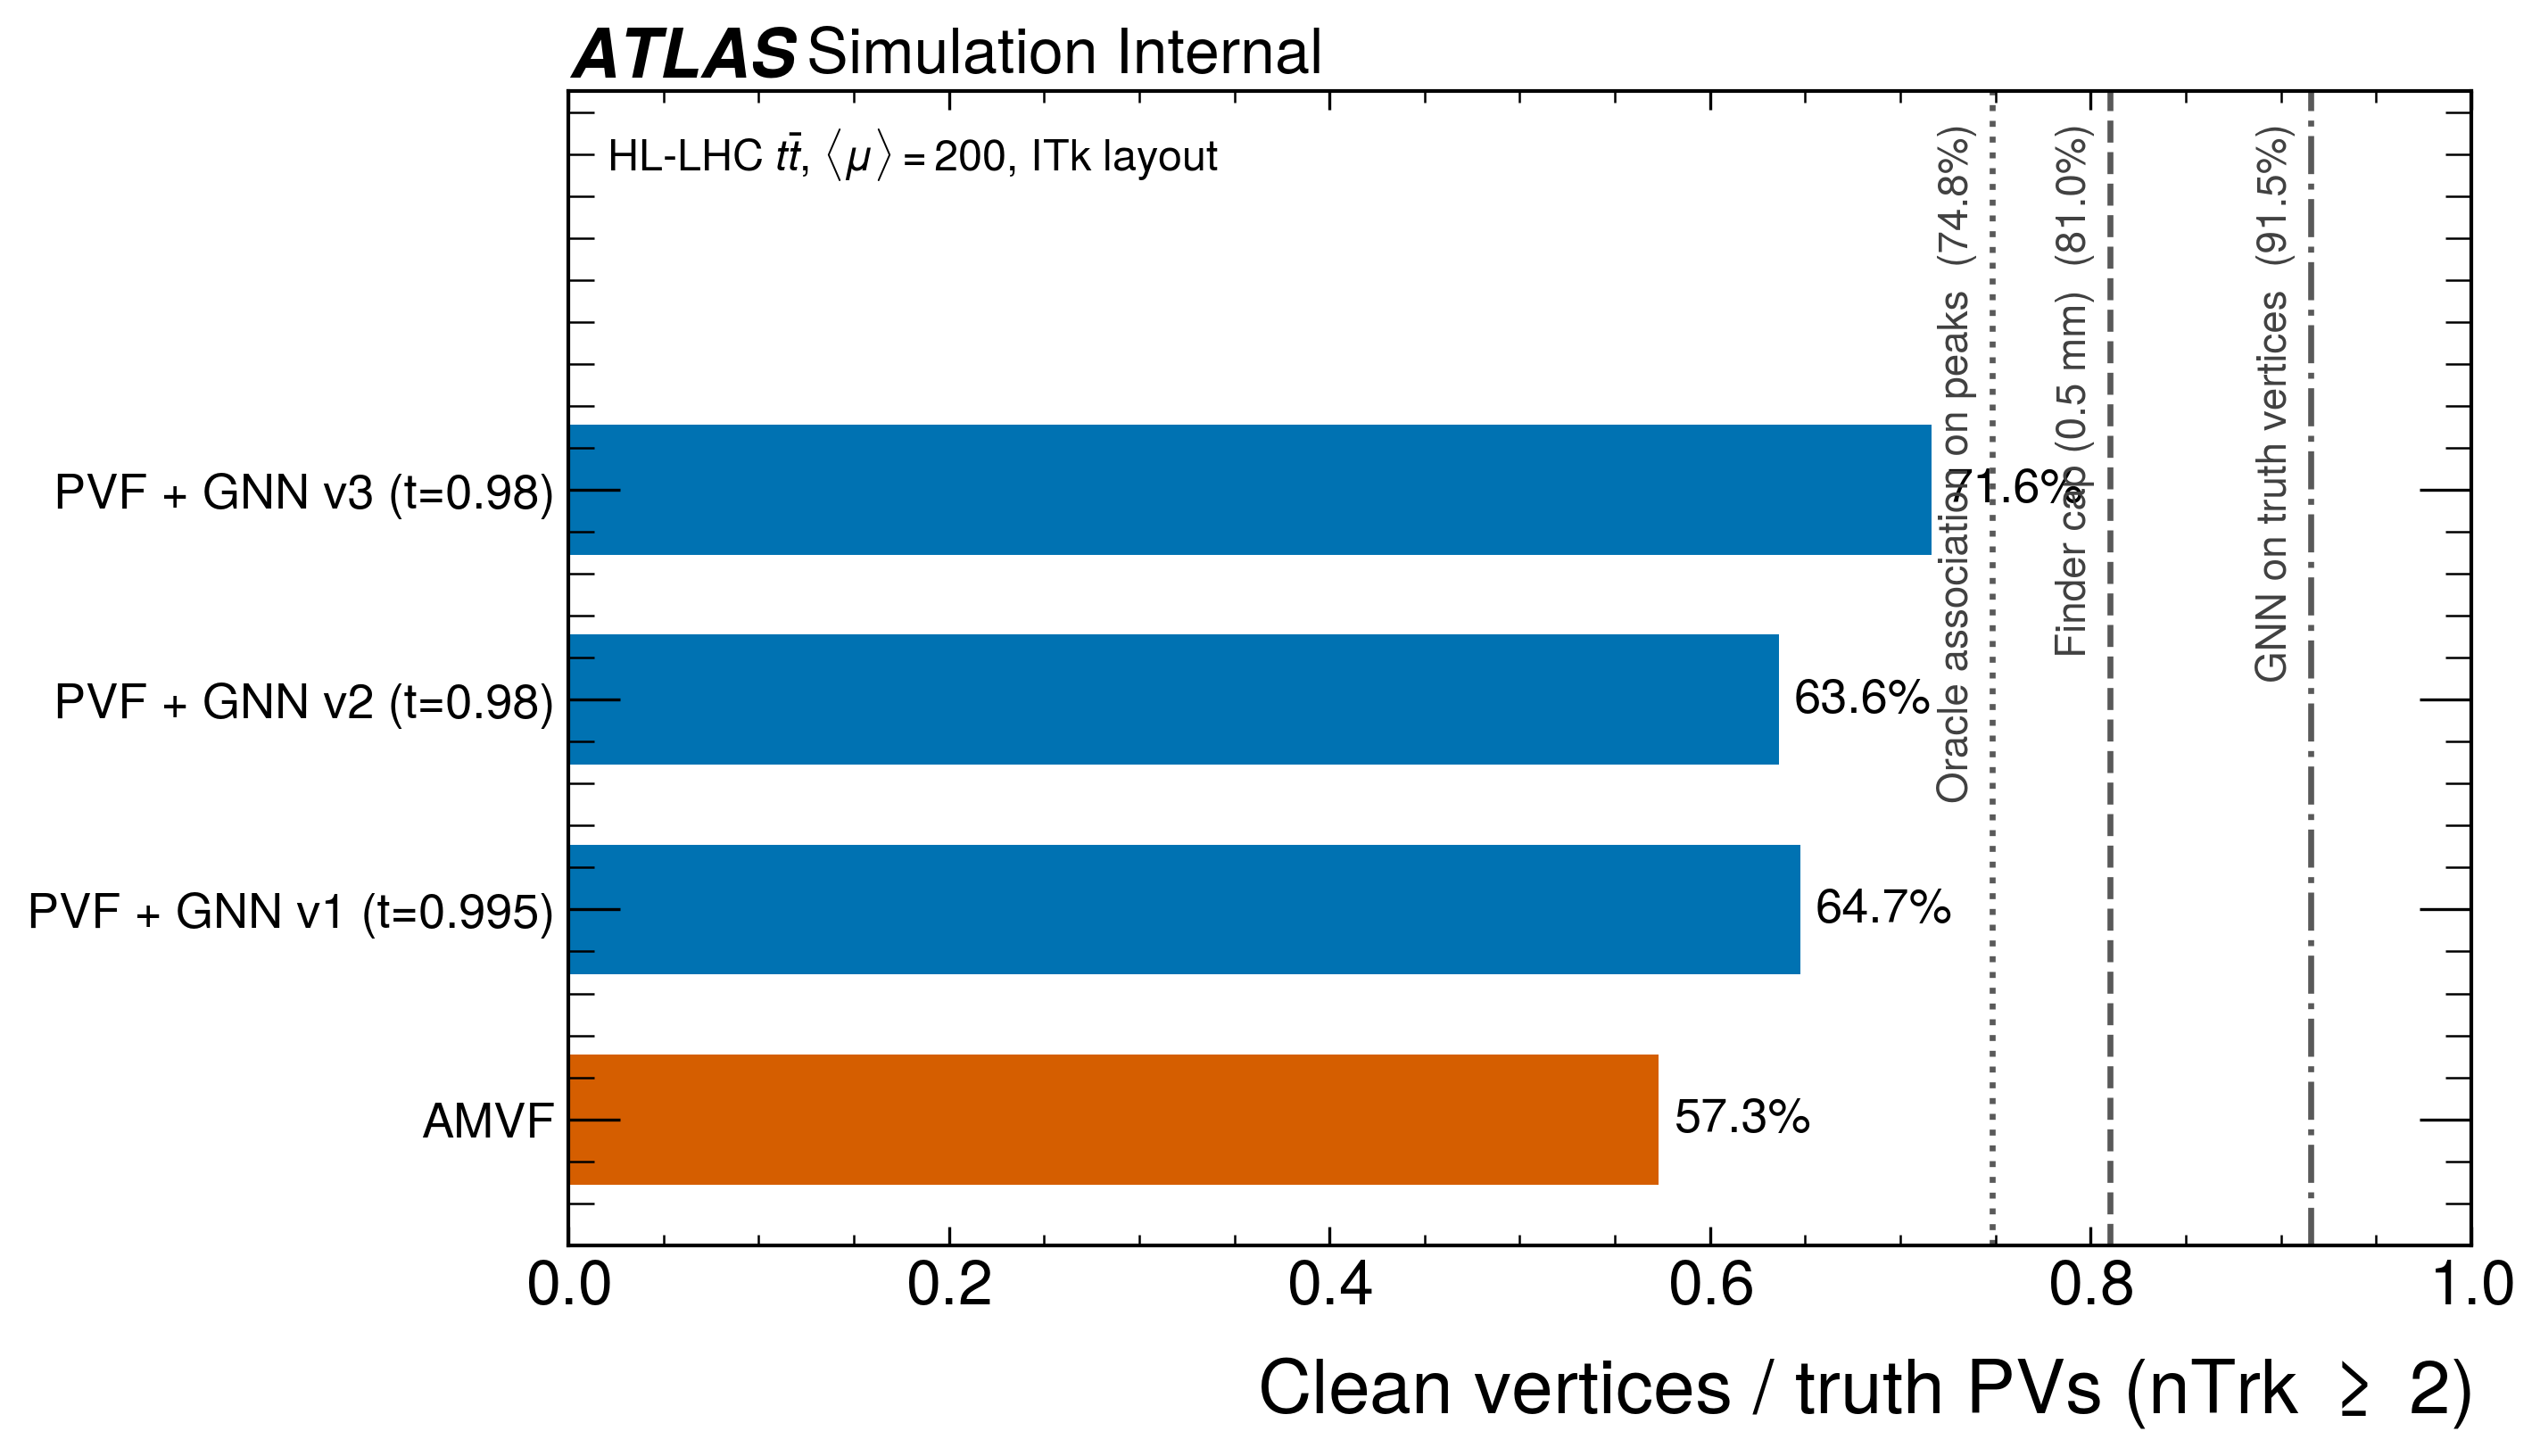
\includegraphics[width=\linewidth, keepaspectratio]{images/pu200_yield_ladder.png}\\[2pt]
            {\scriptsize\textcolor{black!55}{PU200, 1500 events: PV-Finder + GNN vs AMVF, with bounds}}
        \end{column}
    \end{columns}
\end{frame}

\begin{frame}{TTVA I: What It Is and Why We Need It}
    \textbf{Vertex finding tells us \emph{where} the vertices are -- not \emph{which tracks belong to which vertex}.}
    \vspace{0.5em}
    \begin{center}
        tracks \(\;\to\;\) PV-Finder histogram \(\;\to\;\) peak finding \(\;\to\;\) candidate vertices
        \(\;\to\;\) \textcolor{pennred}{\textbf{TTVA}} \(\;\to\;\) per-vertex track lists
    \end{center}
    \vspace{0.5em}
    \begin{columns}[t]
        \begin{column}{0.5\linewidth}
            \textbf{Why analyses need the track lists:}
            \begin{itemize}
                \setlength\itemsep{0.4em}
                \item Hard-scatter choice = vertex with largest \(\sum p_T^2\) of \emph{its tracks}
                \item Pile-up jet rejection cuts on track--vertex association
                \item Any per-vertex quantity (multiplicity, mass, pointing)
            \end{itemize}
        \end{column}
        \begin{column}{0.5\linewidth}
            \textbf{Why we need it for our own results:}
            \begin{itemize}
                \setlength\itemsep{0.4em}
                \item AMVF gets track lists for free from its fit; PV-Finder does not
                \item With TTVA, both chains are judged by the \emph{same} track-based purity criteria -- a genuinely fair comparison
                \item Key design choice: \textbf{train on MC truth vertices} (labels exist), \textbf{deploy on PV-Finder peaks}
            \end{itemize}
        \end{column}
    \end{columns}
\end{frame}

\begin{frame}{TTVA II: The Event as a Graph}
    \begin{columns}[c]
        \begin{column}{0.52\linewidth}
            Each event becomes a \textbf{bipartite graph} with two node types:
            \begin{itemize}
                \setlength\itemsep{0.35em}
                \item \textcolor{mydarkblue}{\textbf{Track nodes}} (8 features): \(d_0,\, z_0,\, \sigma_{d_0},\, \sigma_{z_0},\, \mathrm{cov},\, \theta,\, \phi,\, p_T\)
                \item \textcolor{myorange}{\textbf{Vertex nodes}} (2 features): \(z\) position, peak height
                \item \textbf{Edges} = (track, vertex) pairs, each carrying 3 physics attributes:
                \[
                  \frac{z_0 - z_{PV}}{\sqrt{\sigma_{z_0}^2+\sigma_{PV}^2}},\qquad
                  \frac{d_0}{\sigma_{d_0}},\qquad |z_0 - z_{PV}|
                \]
                \item Training label: edge = 1 iff MC truth says the track came from that vertex
            \end{itemize}
        \end{column}
        \begin{column}{0.46\linewidth}
            \centering
            \begin{tikzpicture}[x=0.85cm, y=0.85cm]
                \foreach \y/\n in {3.6/1, 2.4/2, 1.2/3, 0.0/4} {
                    \filldraw[fill=mydarkblue!14, draw=mydarkblue!70, thick] (0,\y) circle (8pt)
                        node[font=\scriptsize] {\(t_\n\)};
                }
                \foreach \y/\n in {3.0/1, 1.8/2, 0.6/3} {
                    \filldraw[fill=myorange!20, draw=myorange!80!black, thick] (4,\y) circle (8pt)
                        node[font=\scriptsize] {\(v_\n\)};
                }
                \foreach \s/\t in {3.6/3.0, 3.6/1.8, 2.4/3.0, 2.4/1.8, 1.2/1.8, 1.2/0.6, 0.0/1.8, 0.0/0.6} {
                    \draw[black!40, thick] (0.3,\s) -- (3.7,\t);
                }
                \draw[pennred, very thick] (0.3,2.4) -- (3.7,3.0);
                \node[font=\tiny, text=pennred] at (2.0,3.35) {edge score \(\in[0,1]\)};
                \node[font=\tiny, text=black!55] at (0.0,-0.75) {tracks};
                \node[font=\tiny, text=black!55] at (4.0,-0.75) {candidate vertices};
            \end{tikzpicture}\\[6pt]
            {\scriptsize At PU200: \(\sim\)930 tracks \(\times\) 128 vertices \(\to\) each track keeps its \(k=20\)
            nearest vertices in \(|\Delta z|\) (retains 99.5\% of true edges, \(\sim\)18.5k edges/event).}
        \end{column}
    \end{columns}
\end{frame}

\begin{frame}{TTVA III: The Model -- a Small Graph Attention Network}
    \begin{columns}[c]
        \begin{column}{0.55\linewidth}
            \begin{enumerate}
                \setlength\itemsep{0.45em}
                \item Embed track (8) and vertex (2) features into 32 dimensions
                \item \textbf{2 rounds of message passing} (graph attention, 4 heads): each node updates from its neighbours, with the edge attributes steering the attention
                \item[] {\small \(\Rightarrow\) a vertex that already attracts many compatible tracks attracts the next one more strongly -- context a per-pair cut cannot express}
                \item A 3-layer MLP on each (track, vertex) embedding pair \(\to\) \textbf{one score per edge}
            \end{enumerate}
            \vspace{0.2em}
            {\footnotesize \textbf{Size and training:} 39\,521 parameters (\(90\times\) smaller than
            PV-Finder), 3.8~ms/event; trained on 180k PU200 events in 3.2~h.}
        \end{column}
        \begin{column}{0.45\linewidth}
            \centering
            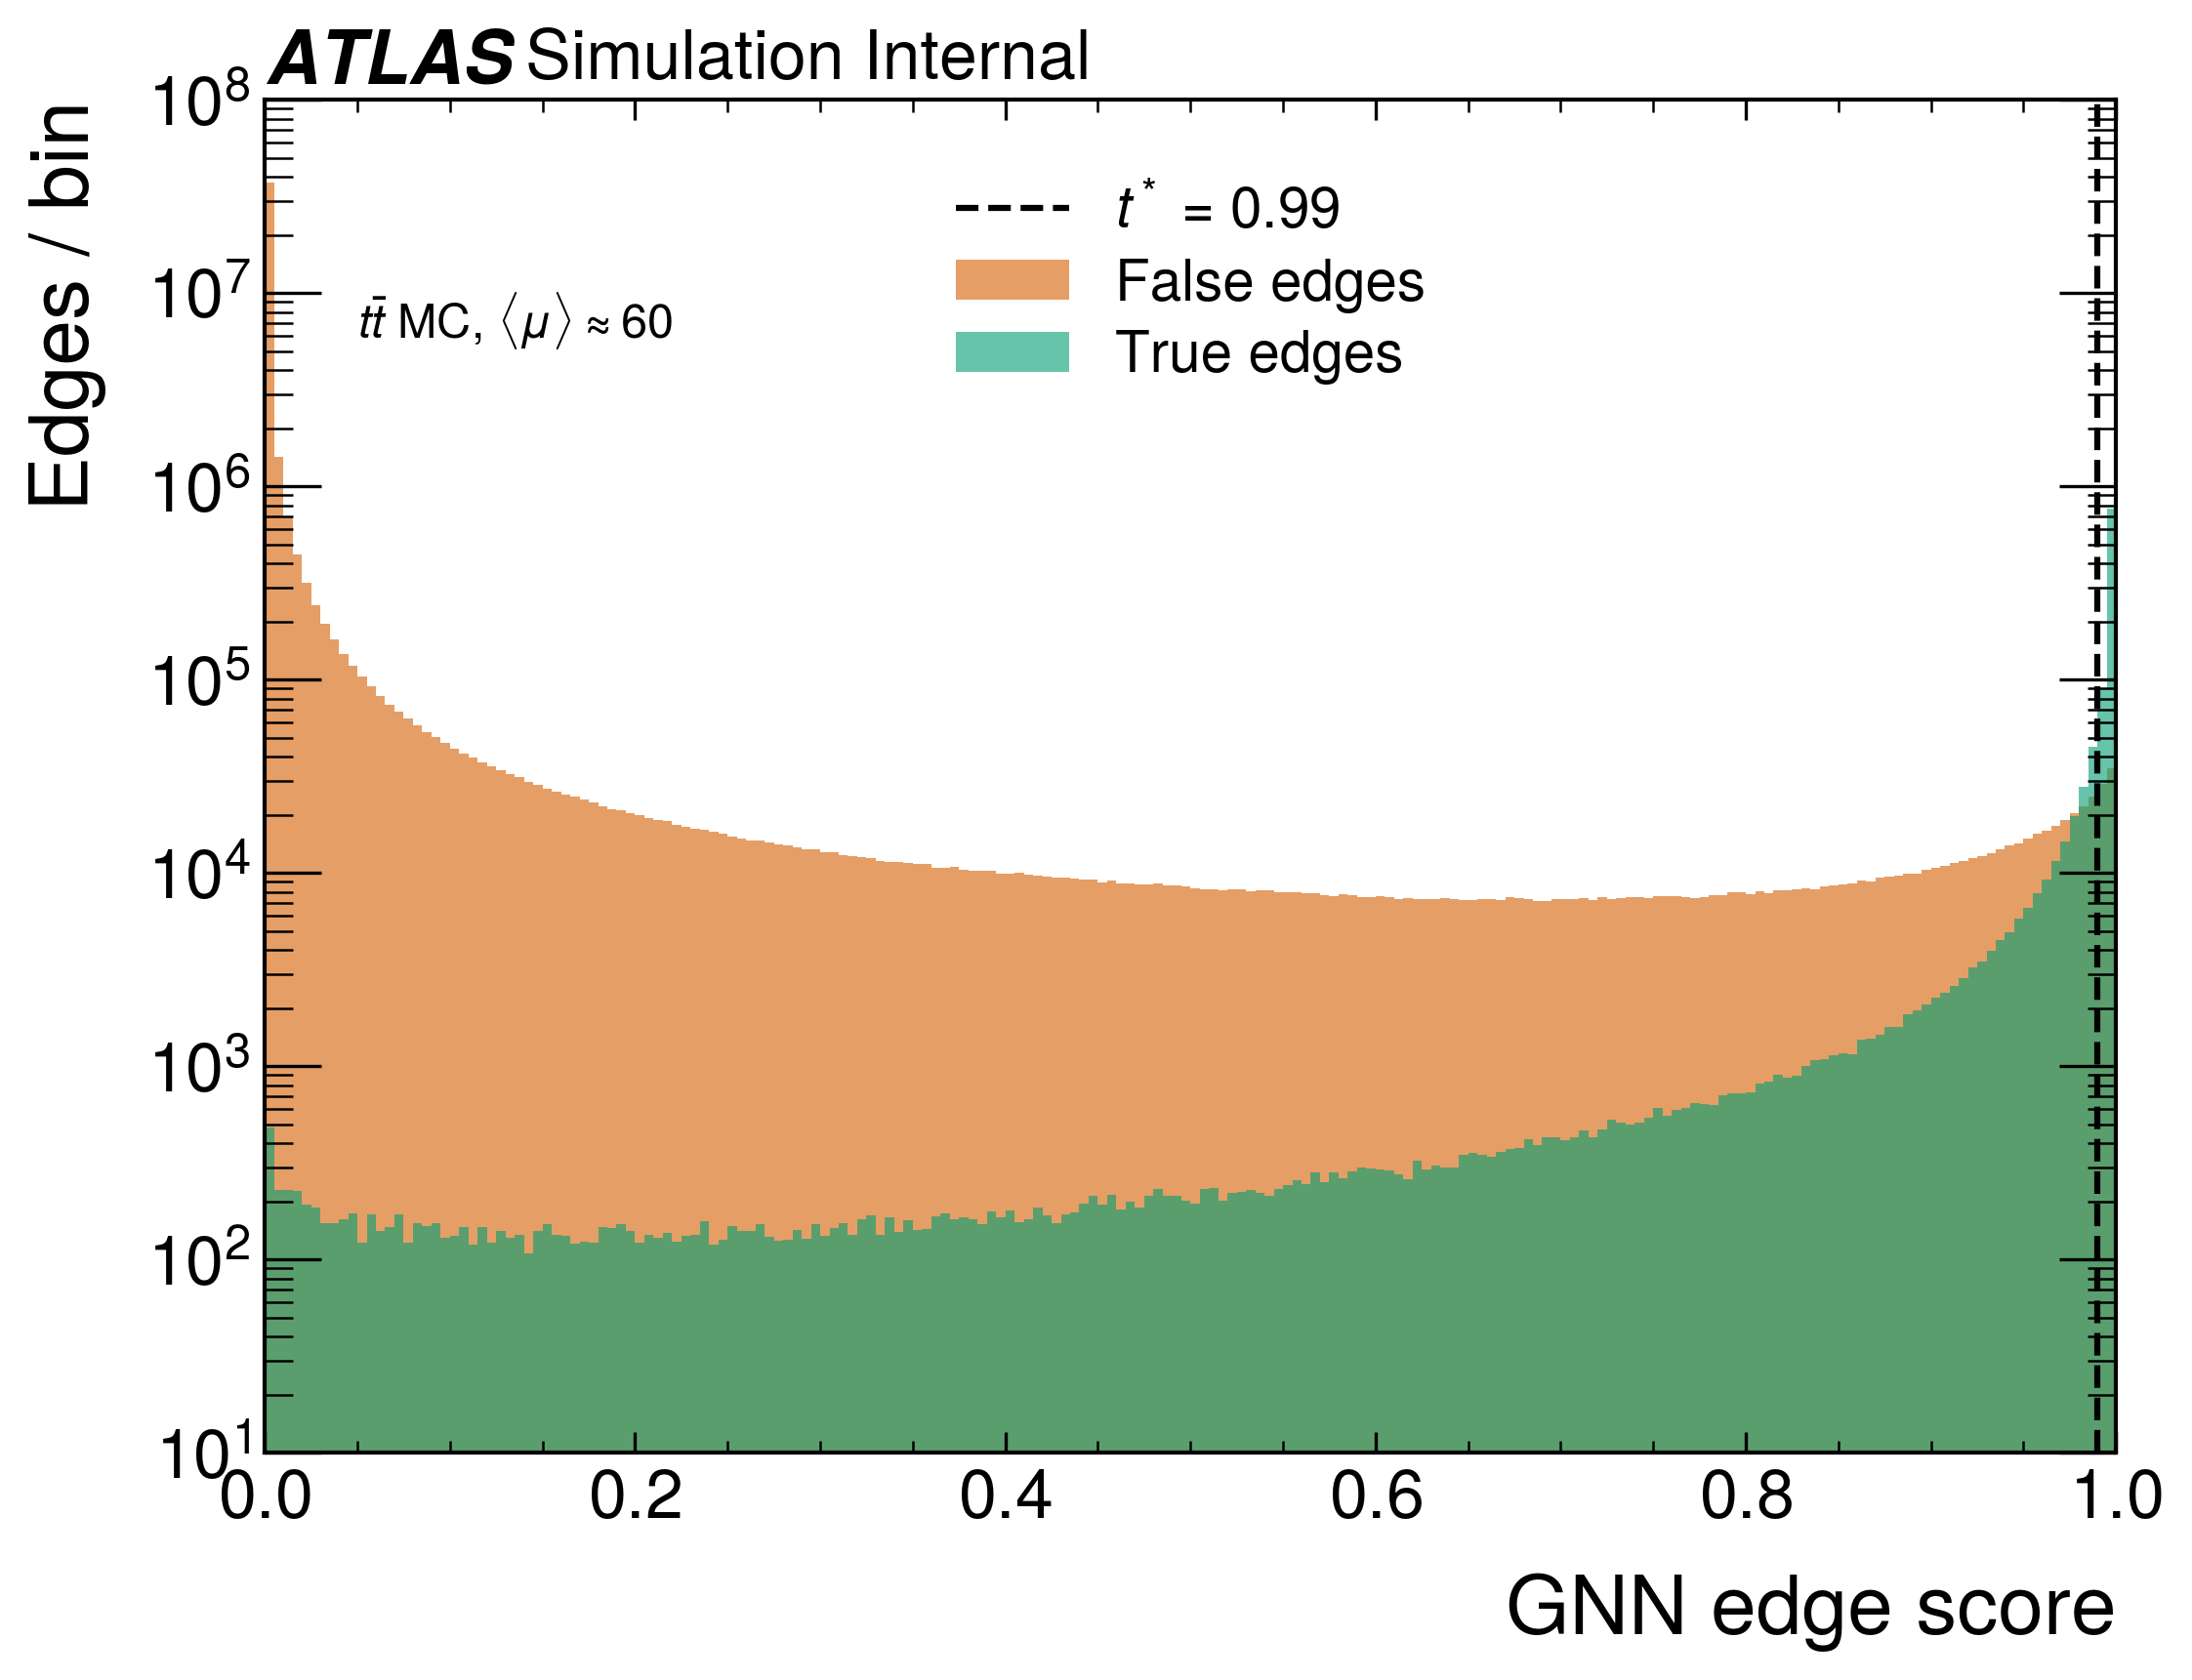
\includegraphics[width=0.94\linewidth, keepaspectratio]{images/edge_score_distributions.png}\\[2pt]
            {\scriptsize\textcolor{black!55}{Edge scores, true vs false edges (\(\mu\approx60\) test set):
            the classifier is nearly saturated -- ROC AUC 0.998 on 45M edges.}}
        \end{column}
    \end{columns}
\end{frame}

\begin{frame}{TTVA IV: From Scores to Vertices}
    \small
    \begin{columns}[c]
        \begin{column}{0.55\linewidth}
            \textbf{Selection (MaxScore):} each track goes to its highest-scoring vertex,
            \emph{only if} that score exceeds a threshold \(t\); otherwise it stays unassigned.
            \begin{itemize}
                \setlength\itemsep{0.3em}
                \item The model runs \textbf{once}; \(t\) is a free post-hoc knob
                \item Scores saturate near 1 \(\to\) working points live at \(t\geq0.9\) (worth +11 points at PU200 vs \(t=0.5\), no retraining)
            \end{itemize}
            \vspace{0.3em}
            \textbf{Vertex categories} from the truth of the assigned tracks
            (headline: \textbf{clean / truth PVs}, \(n_{trk}\geq2\); AMVF through the \emph{identical} classifier):
            \begin{itemize}
                \setlength\itemsep{0.2em}
                \item \textcolor{mygreen}{\textbf{Clean}}: \(\geq50\%\) of tracks from one truth vertex
                \item \textcolor{myorange}{\textbf{Merged}}: no majority contributor
                \item \textcolor{myblue}{\textbf{Split}}: truth vertex already claimed by a larger vertex
                \item \textcolor{myred}{\textbf{Fake}}: no assigned track has any truth vertex
            \end{itemize}
        \end{column}
        \begin{column}{0.45\linewidth}
            \centering
            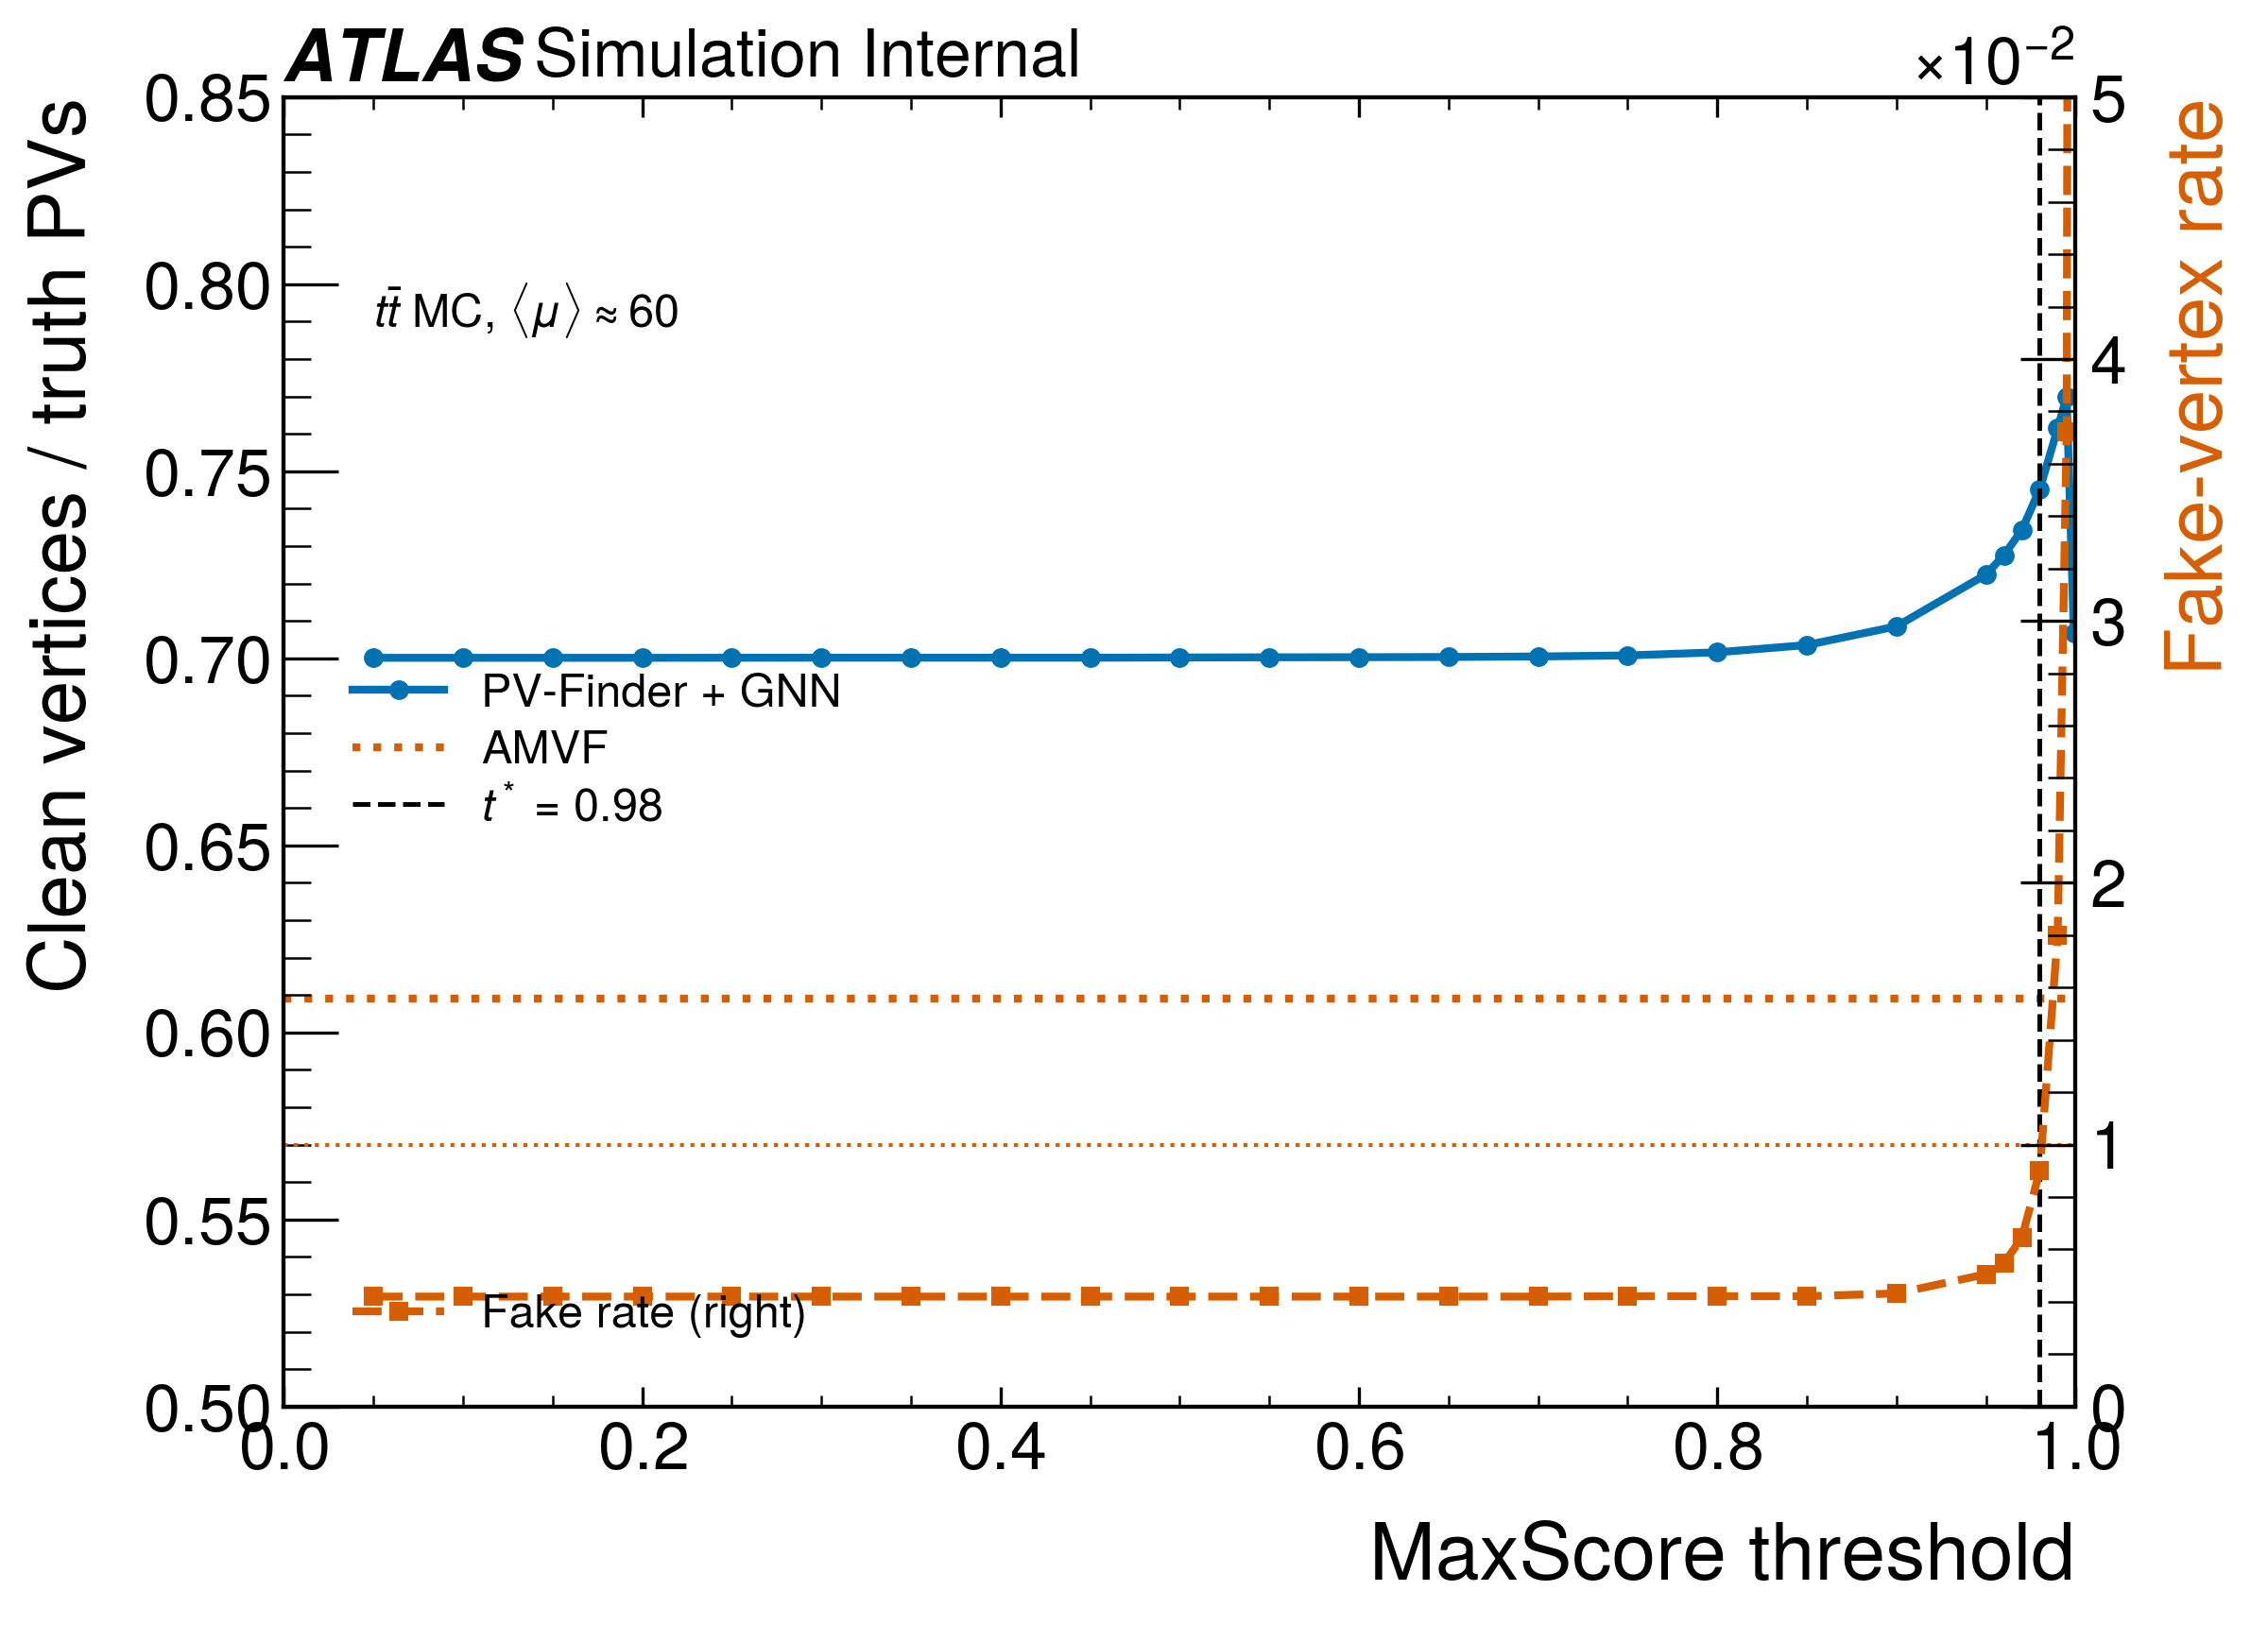
\includegraphics[width=0.94\linewidth, keepaspectratio]{images/clean_efficiency_vs_threshold.png}\\[2pt]
            {\scriptsize\textcolor{black!55}{\(\mu\approx60\) threshold scan: the working point \(t=0.99\)
            gives 77.4\% at a 0.02\% fake rate.}}\\[3pt]
            {\scriptsize \textbf{Convention fix:} zero-track vertices are dropped, not booked as Fake
            (clean/truth provably unchanged) -- unlocks higher \(t\).}
        \end{column}
    \end{columns}
\end{frame}

\begin{frame}{TTVA V: Results at \(\mu\approx60\) (MC, 2550 events)}
    \begin{columns}[c]
        \begin{column}{0.5\linewidth}
            \centering
            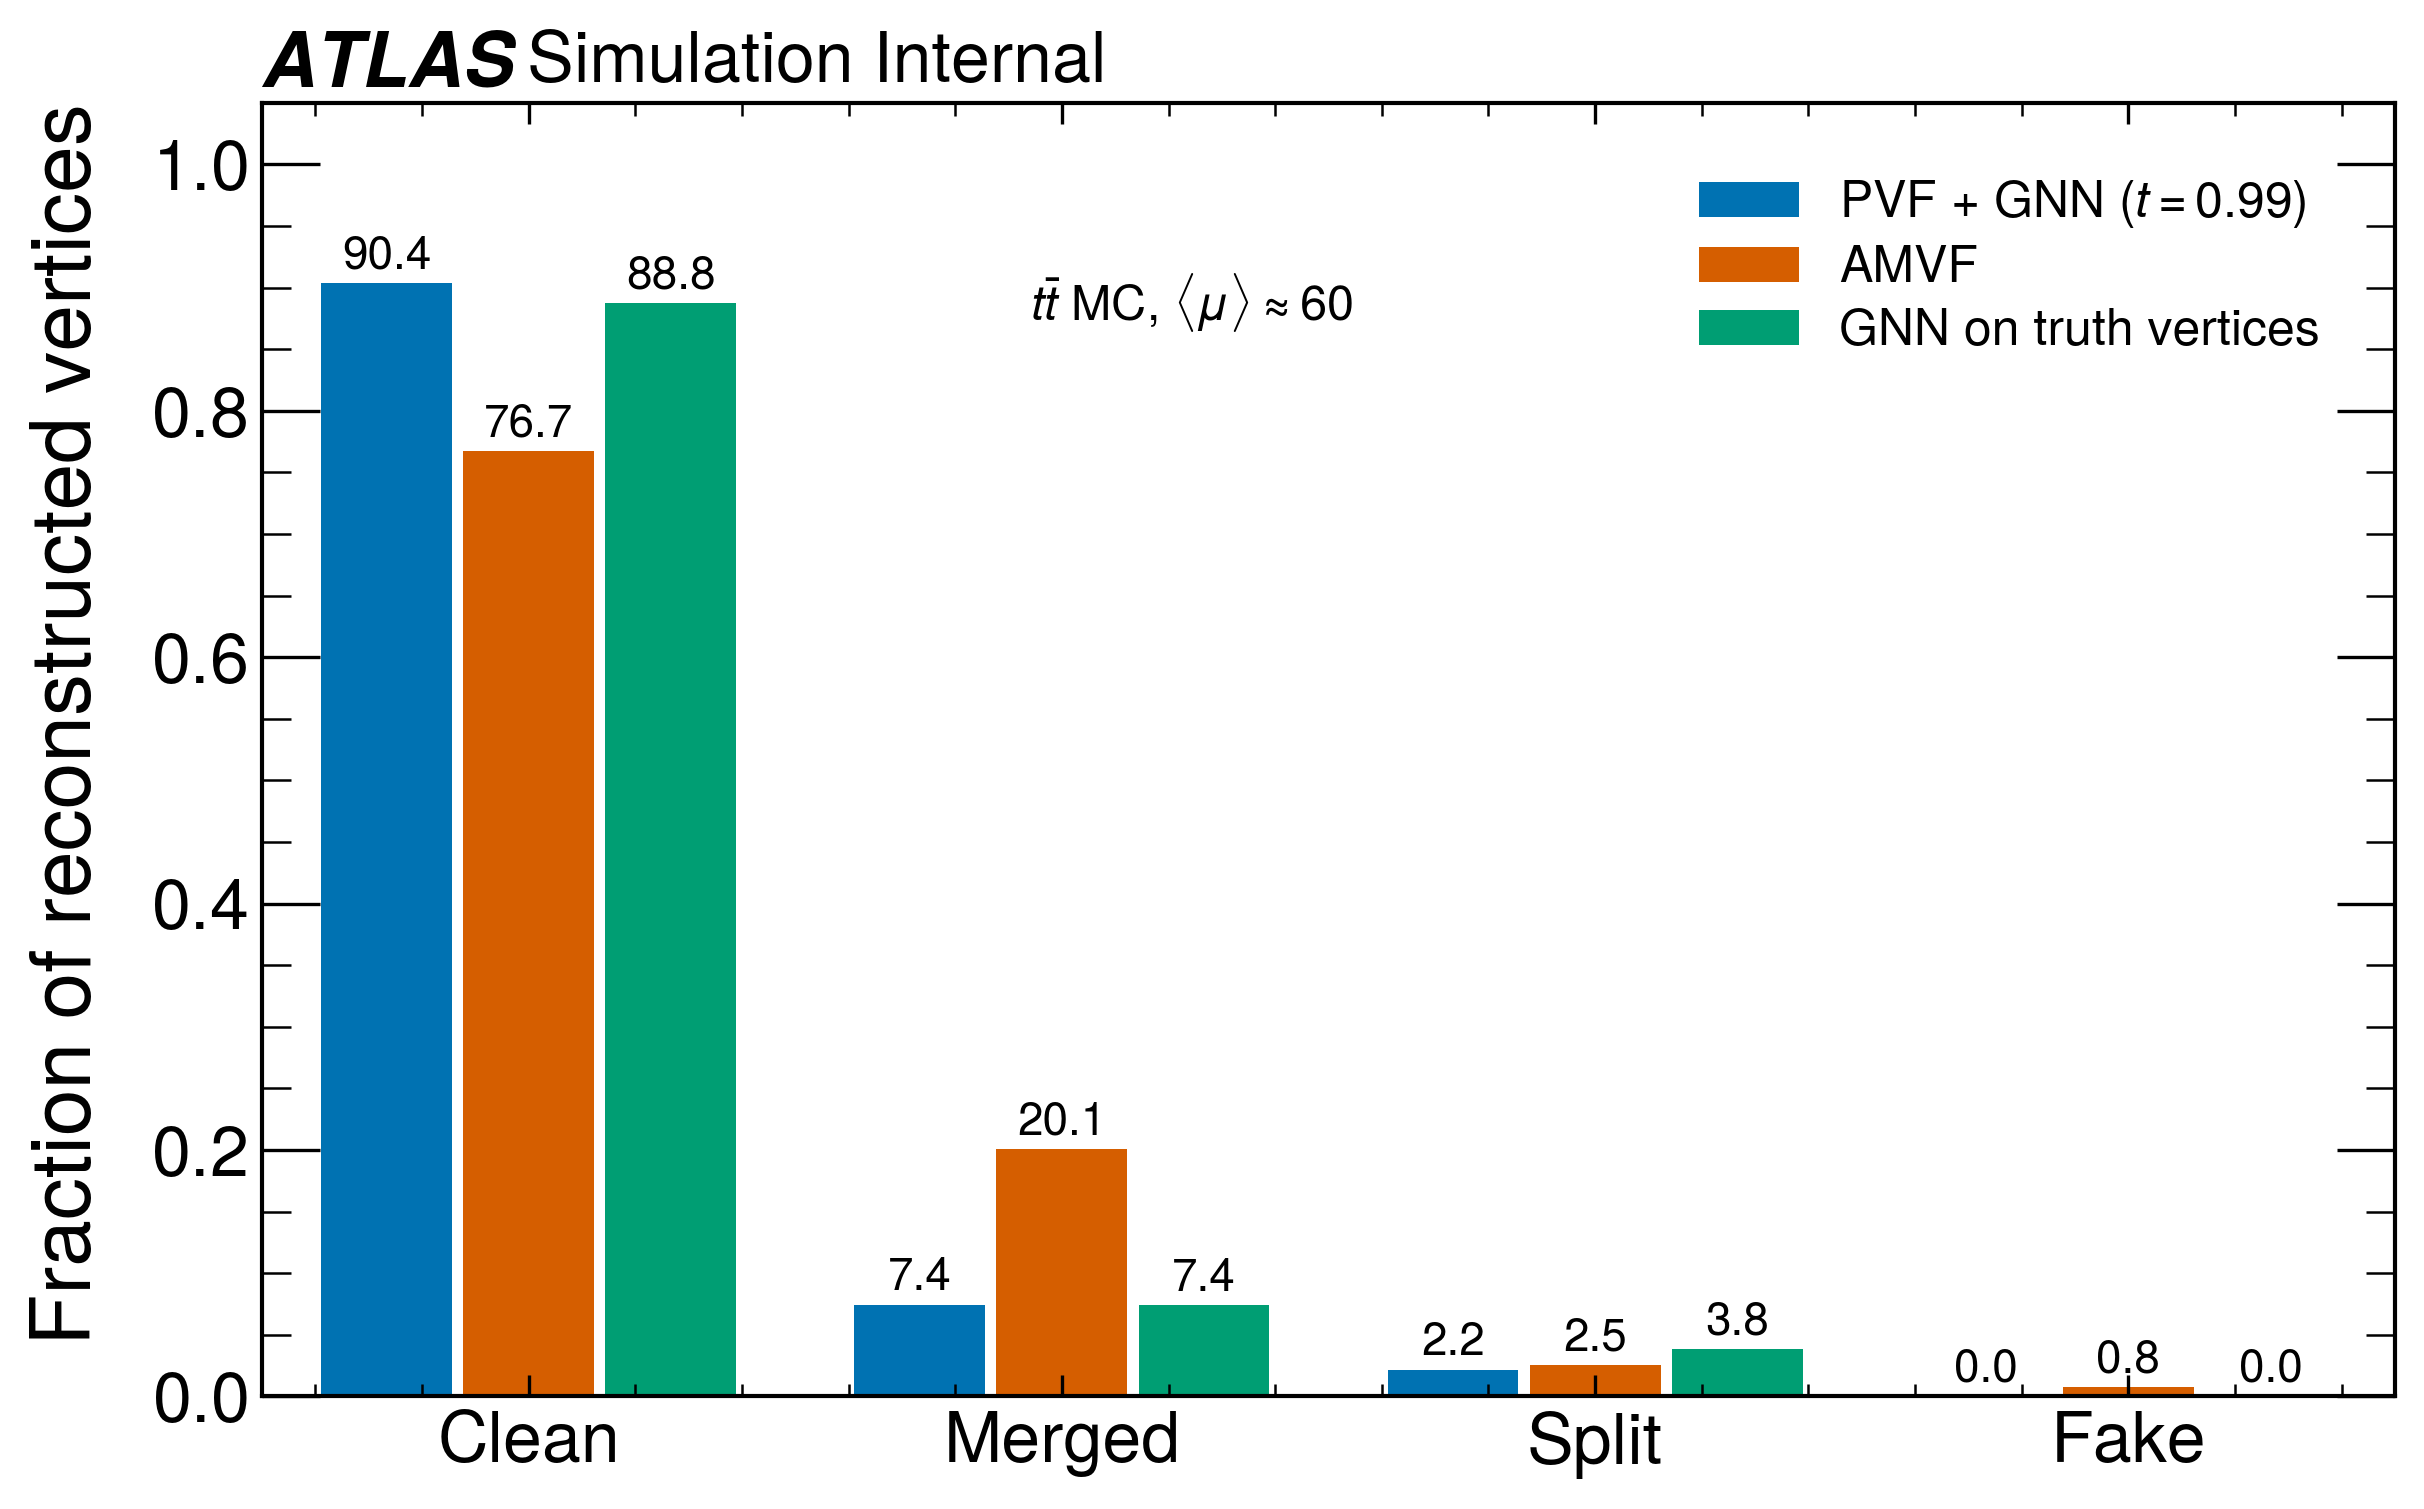
\includegraphics[width=\linewidth, keepaspectratio]{images/category_rates.png}
        \end{column}
        \begin{column}{0.5\linewidth}
            \centering
            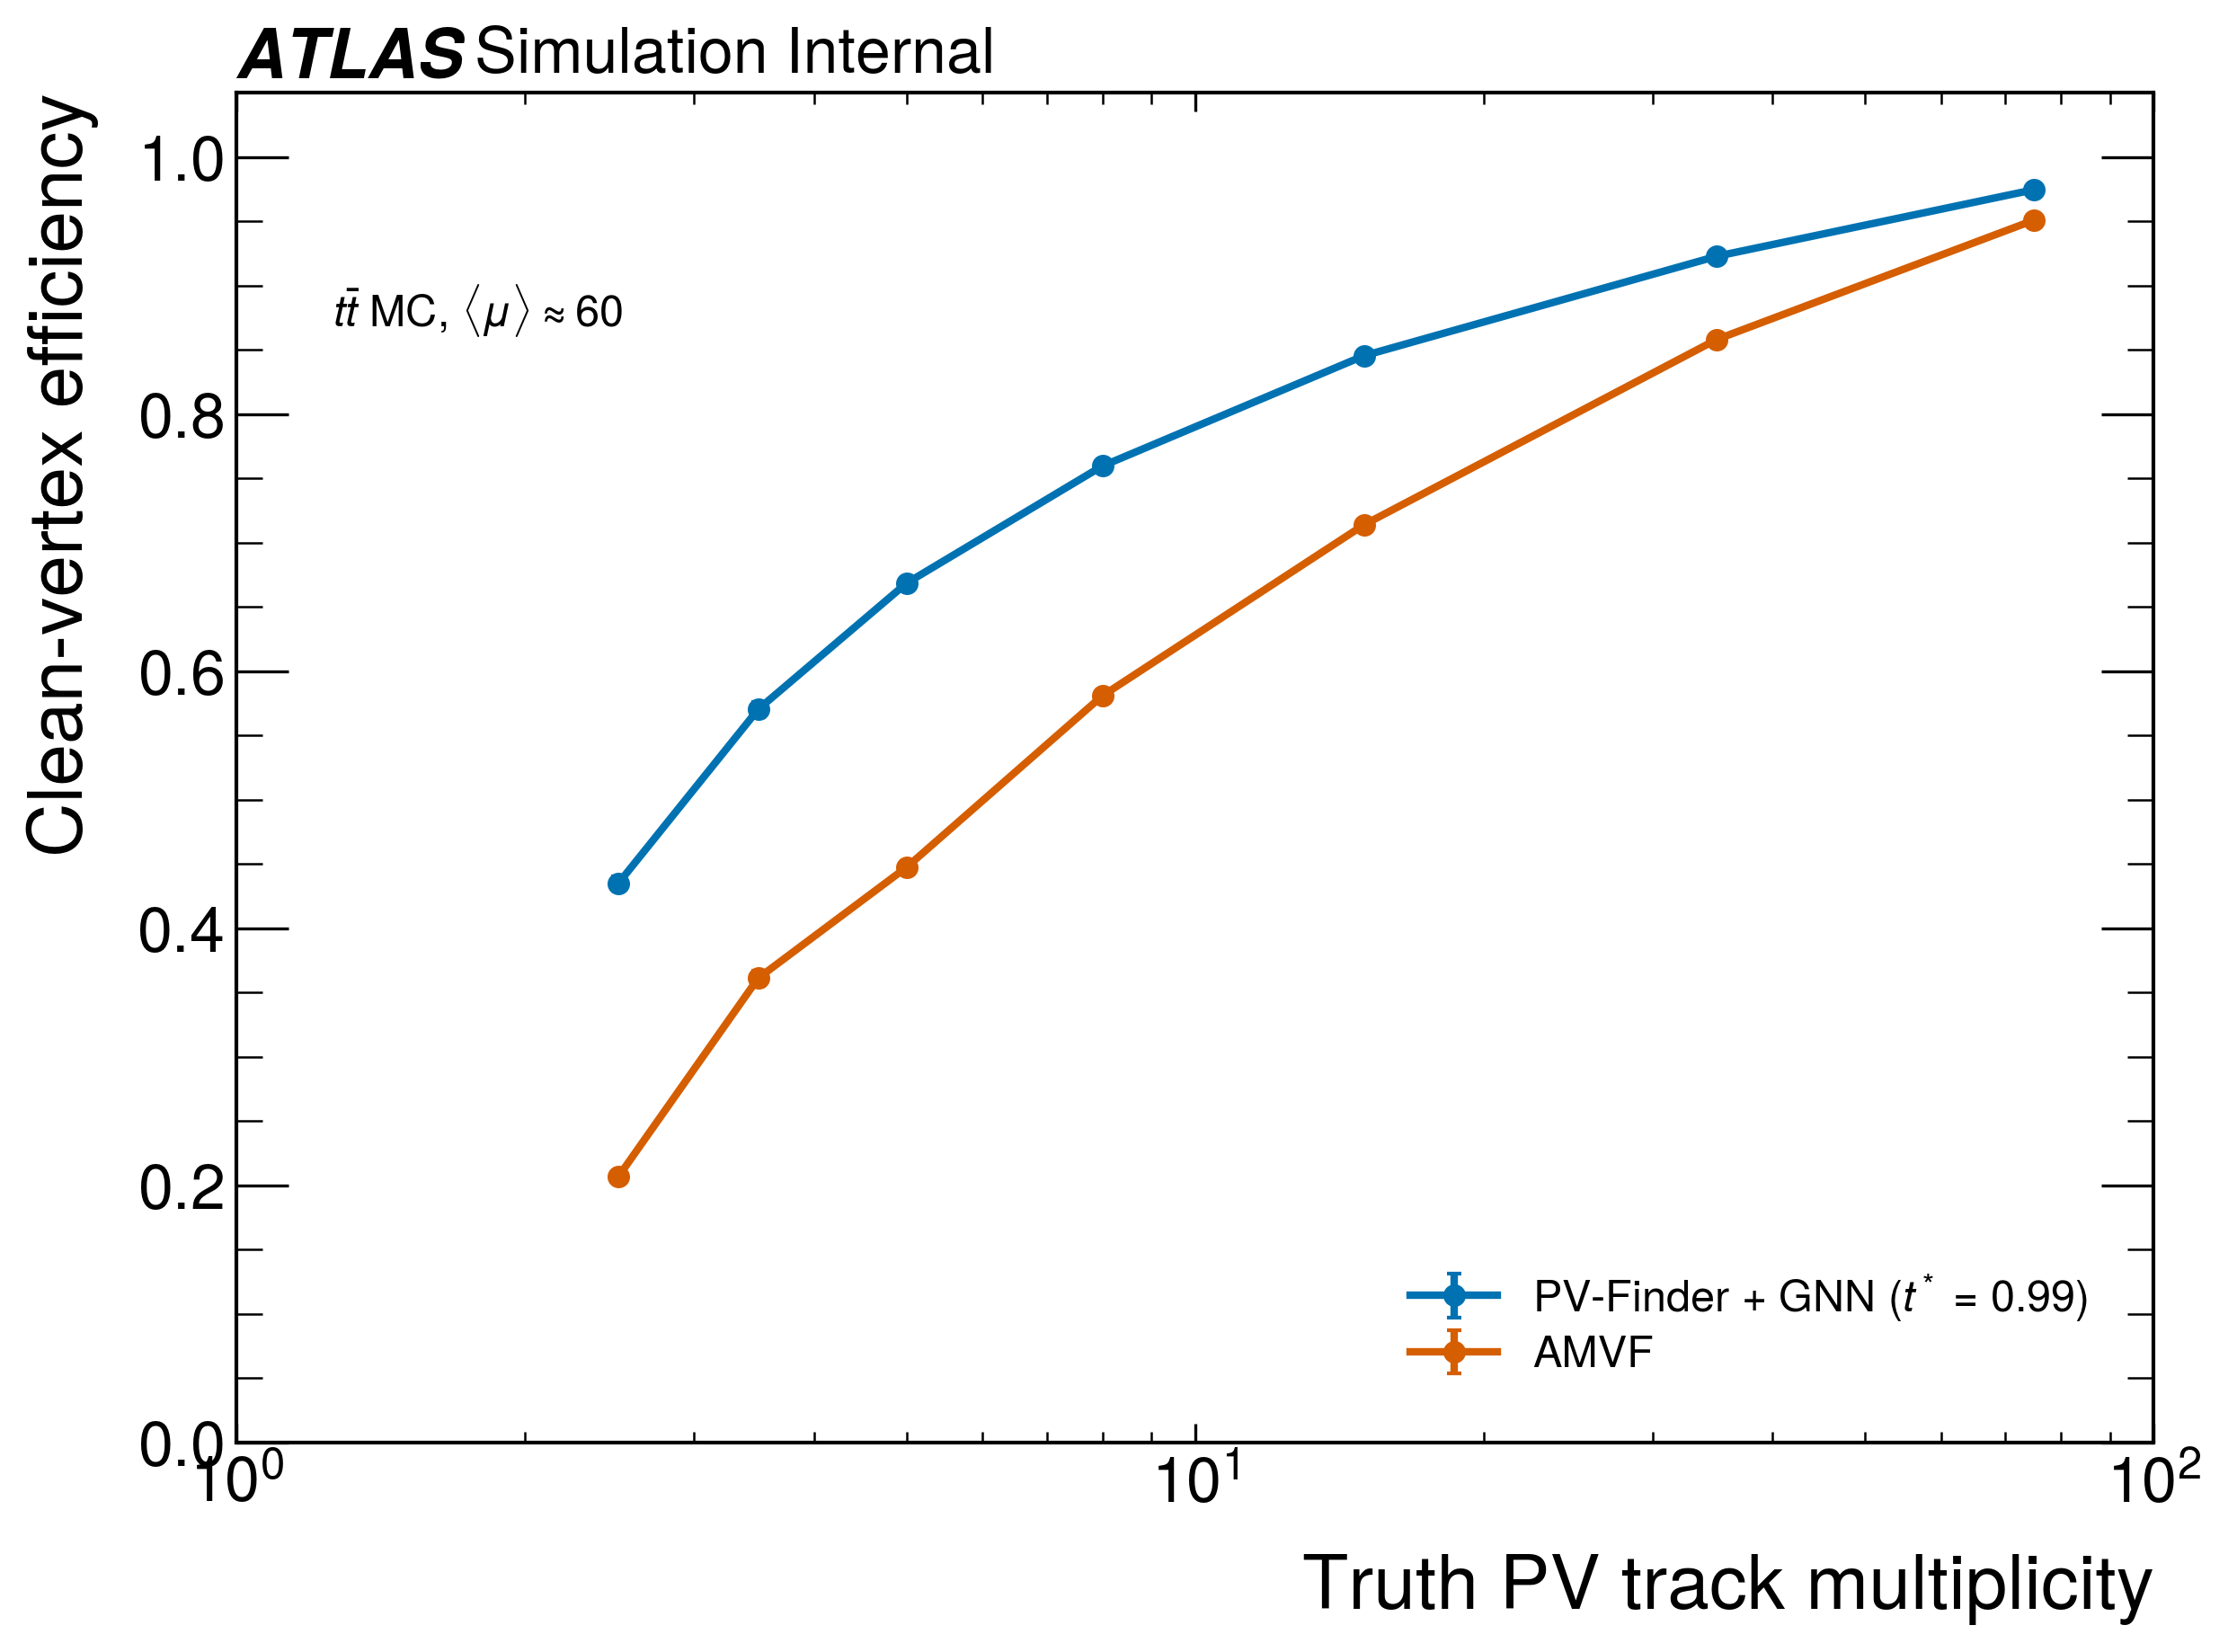
\includegraphics[width=\linewidth, keepaspectratio]{images/clean_efficiency_vs_ntracks.png}
        \end{column}
    \end{columns}
    \vspace{0.4em}
    \centering
    \begin{tabular}{lcccc}
        \textbf{Chain} & Clean & Merged & Fake & \textbf{Clean/truth} \\
        \hline
        PV-Finder peaks + GNN (current, \(t=0.99\)) & 90.4\% & 7.4\% & 0.02\% & \textbf{77.4\%} \\
        \quad legacy training, \(t=0.995\) & 86.8\% & 8.2\% & 0.01\% & 77.0\% \\
        AMVF & 76.7\% & 20.0\% & 0.7\% & 60.9\% \\
    \end{tabular}\\[3pt]
    {\footnotesize Above AMVF in \emph{every} multiplicity bin; track-level \(F_1\) 0.874 vs 0.849; HS-ID 99.0\% vs 98.8\%.}
\end{frame}

\begin{frame}{TTVA VI: Run 3 Collision Data (truth-free check)}
    \begin{columns}[c]
        \begin{column}{0.55\linewidth}
            No truth on data \(\to\) use AMVF as a reference, not as truth:
            \begin{itemize}
                \setlength\itemsep{0.5em}
                \item \textbf{95.7\%} of tracks assigned by both methods land on the same vertex
                (83.7\% of all AMVF-assigned tracks)
                \item Leading-\(\sum p_T^2\) (hard-scatter proxy) vertex agrees in \textbf{88.7\%} of events
                \item The GNN assigns 83\% of tracks on data vs AMVF's 95\%: it abstains more on data, and agrees with AMVF on what it does assign
            \end{itemize}
        \end{column}
        \begin{column}{0.45\linewidth}
            \begin{itemize}
                \setlength\itemsep{0.5em}
                \item Score distributions on data closely track MC
                \item \(\sim3\times\) more tracks at intermediate scores: more ambiguous tracks on real data
                -- a mild, visible domain shift, consistent with the larger unassigned fraction
                \item Full PVF (T2KDE+K2H) \(\to\) peaks \(\to\) GNN chain runs unchanged on data
            \end{itemize}
        \end{column}
    \end{columns}
\end{frame}

\begin{frame}{TTVA VII: HL-LHC Full Chain -- Where Does the Yield Go?}
    \begin{columns}[c]
        \begin{column}{0.55\linewidth}
            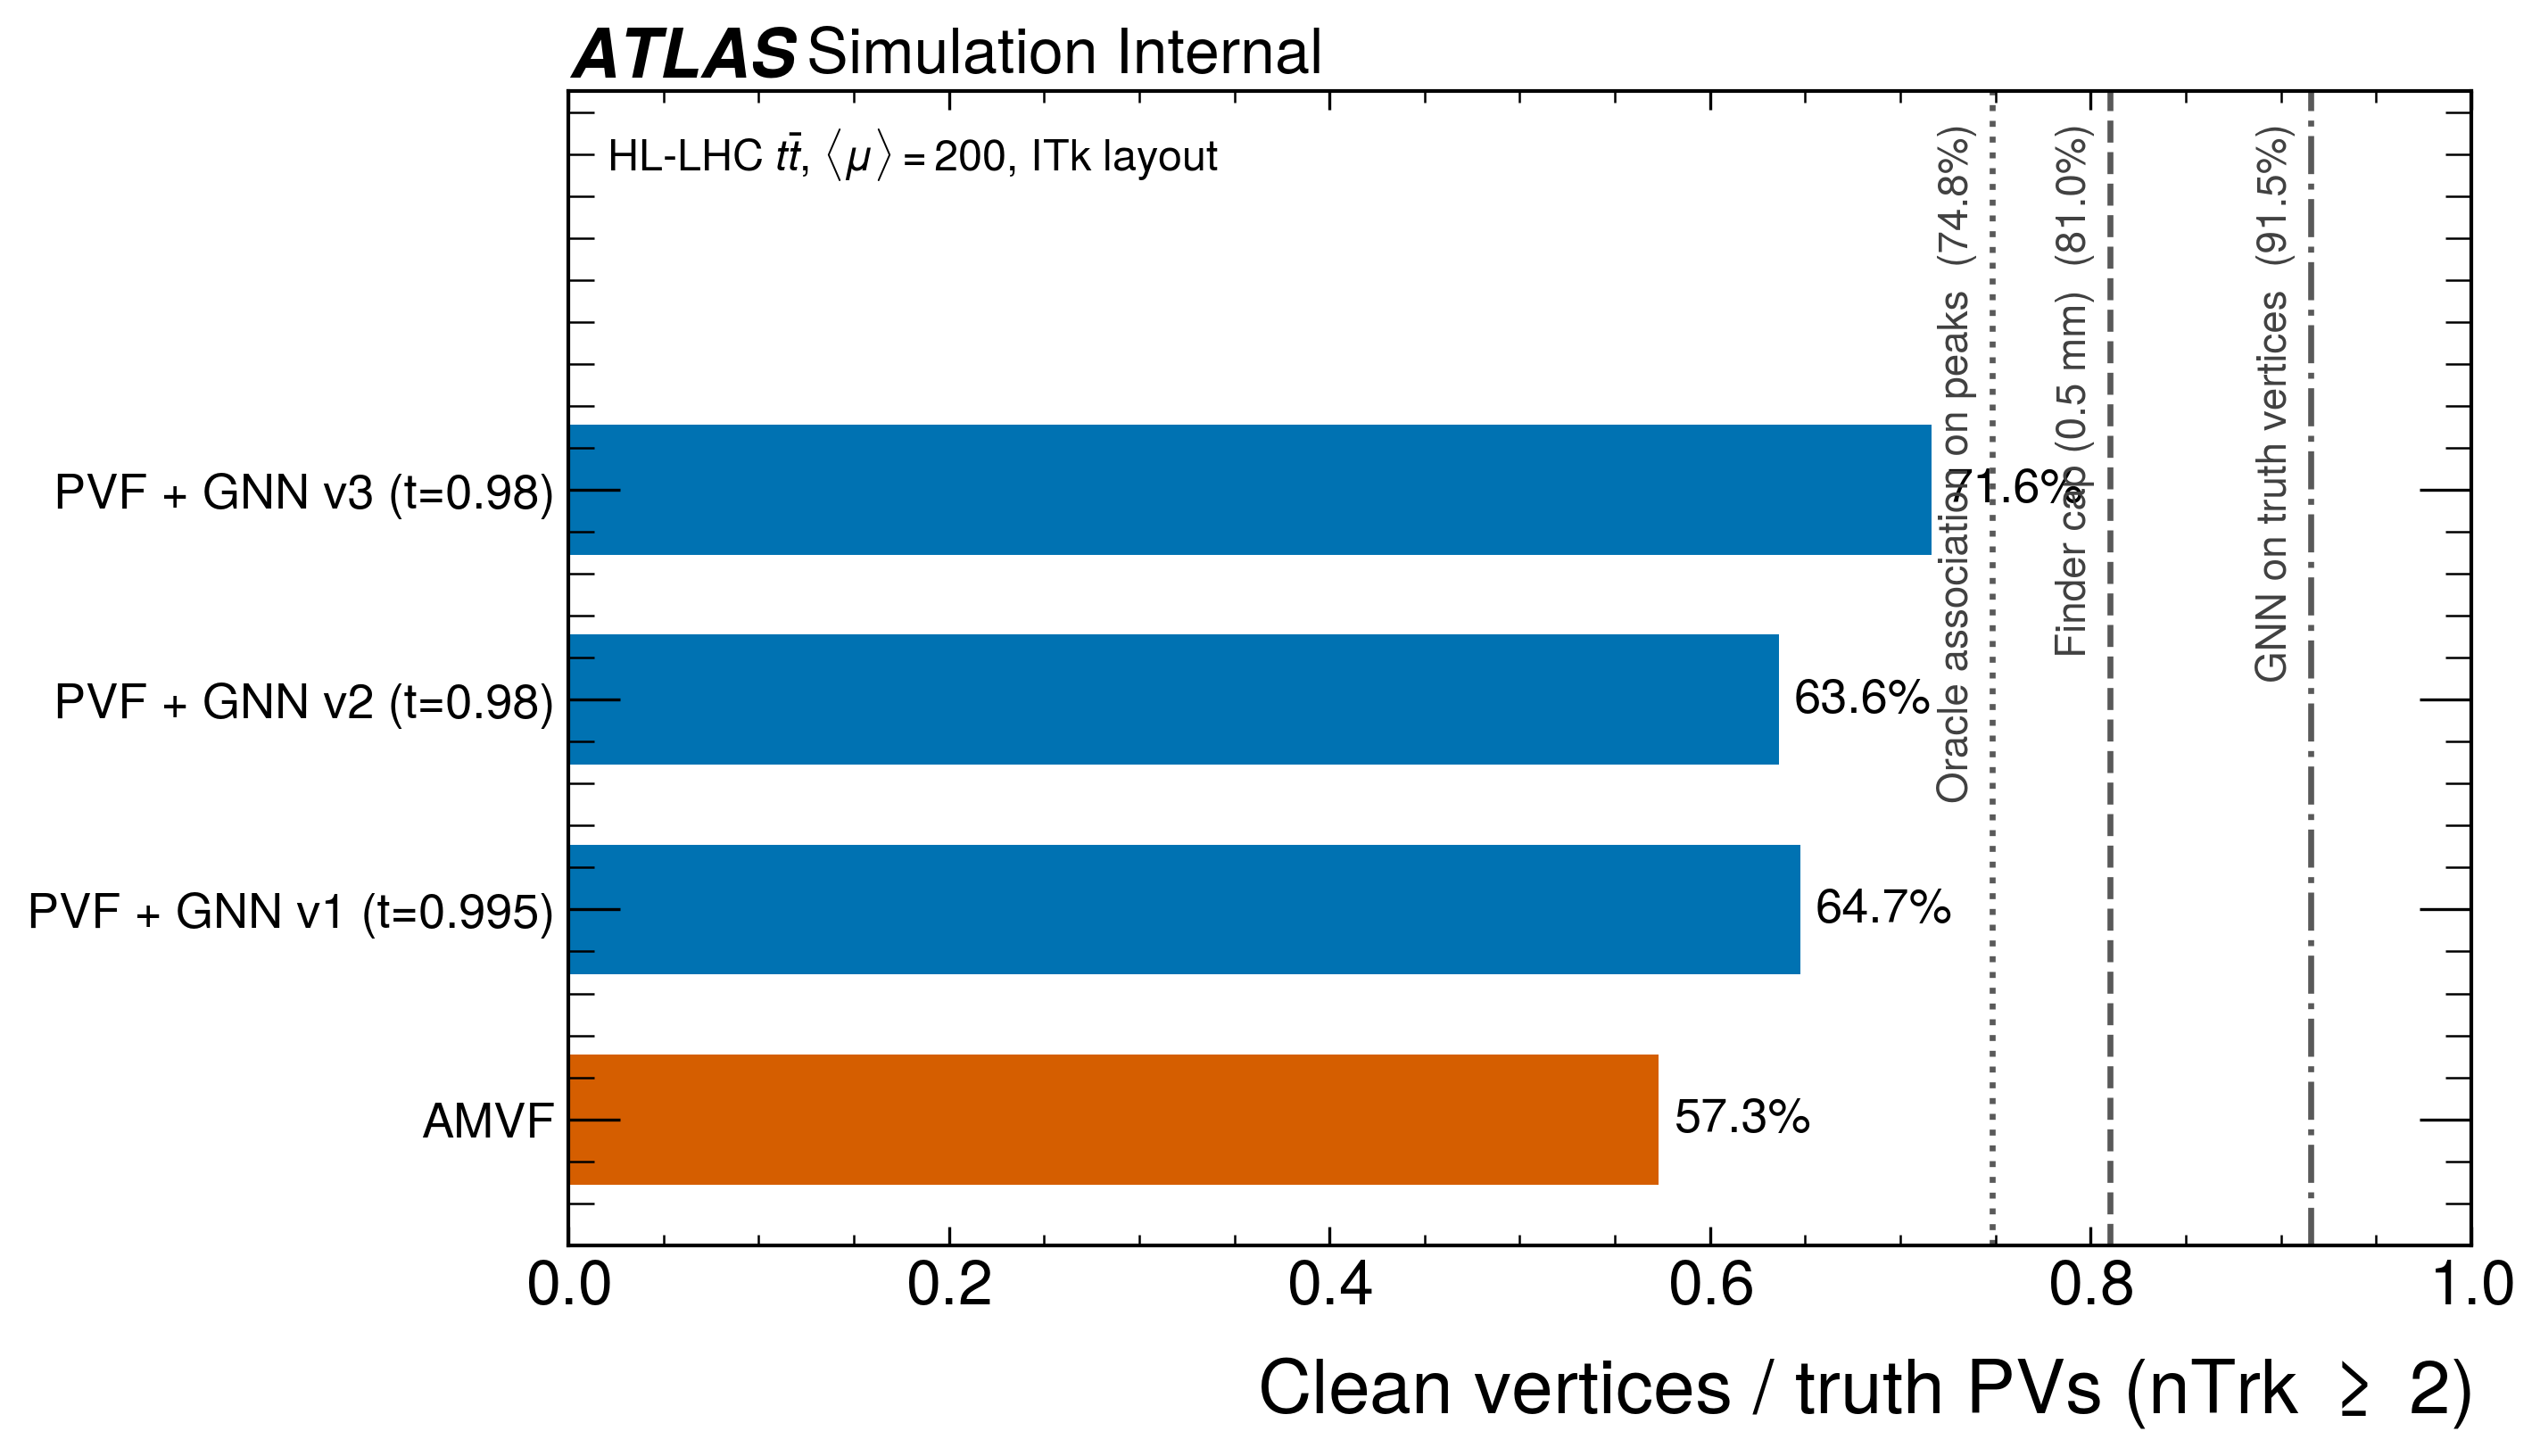
\includegraphics[width=\linewidth, keepaspectratio]{images/pu200_yield_ladder.png}
        \end{column}
        \begin{column}{0.45\linewidth}
            Decomposition on 1500 events (148k truth PVs):
            \begin{itemize}
                \setlength\itemsep{0.4em}
                \item \textbf{Finder cap 81.0\%}: truth PVs with a peak within 0.5~mm -- misses are
                low-multiplicity (median \(n_{trk}=3\); see backup miss-vs-\(n_{trk}\) plot)
                \item \textbf{Oracle 74.8\%}: assign every track to the peak nearest its \emph{true} vertex --
                the 6-point drop is close pairs sharing one peak, unrecoverable by \emph{any} associator
                \item \textbf{GNN (current): 71.6\%} = \textbf{96\% of the oracle} -- the associator is nearly saturated;
                what remains belongs to the finder
            \end{itemize}
        \end{column}
    \end{columns}
\end{frame}

\begin{frame}{TTVA VIII: The Truth\(\to\)Peak Transfer Gap (found and closed)}
    \small
    \begin{columns}[c]
        \begin{column}{0.55\linewidth}
            Train on truth vertices, deploy on peaks \(\to\) the vertex nodes look different at deployment:
            \begin{enumerate}
                \setlength\itemsep{0.3em}
                \item \textbf{Bookkeeping}: empty vertices booked as Fake (fixed by drop-empty)
                \item \textbf{A real bug}: the height recipe evaluated its Gaussian 240~mm off \(\to\)
                \emph{every truth graph ever built had heights \(\equiv0\)}, while peaks carry real heights
                (models trained on the dead input \emph{lose} 5--9 points when heights switch on)
                \item \textbf{Distribution shift}: peak widths 2--5\(\times\) the preset, 9.4\% junk peaks, 19\% missing vertices
            \end{enumerate}
            \vspace{0.25em}
            \textbf{The fix}: heights repaired + truth graphs made \emph{chain-like} at build time
            (drop / jitter / resample widths, heights / inject junk -- all \emph{measured} on the chain,
            zero free parameters) + 180k events.
        \end{column}
        \begin{column}{0.45\linewidth}
            \centering
            
\includegraphics[width=\linewidth, keepaspectratio]{images/pu200_v3_learning_curve.png}\\[2pt]
            {\scriptsize\textcolor{black!55}{Current training: smooth climb past the earlier models
            (evaluated on the same live-height graphs).}}
        \end{column}
    \end{columns}
\end{frame}

\begin{frame}{TTVA IX: Final PU200 Result -- PV-Finder + GNN vs AMVF}
    \begin{columns}[c]
        \begin{column}{0.48\linewidth}
            \centering
            
\includegraphics[width=0.92\linewidth, keepaspectratio]{images/pu200_chain_scan.png}
        \end{column}
        \begin{column}{0.52\linewidth}
            \centering
            \begin{tabular}{lcc}
                & \textbf{Clean/truth} & \textbf{Fake} \\
                \hline
                AMVF & 57.3\% & 0.91\% \\
                PVF + GNN (current, \(t=0.98\)) & \textbf{71.6\%} & \textbf{0.05\%} \\
                \hline
                oracle on these peaks & 74.8\% & --- \\
            \end{tabular}\\[8pt]
            \begin{itemize}
                \setlength\itemsep{0.4em}
                \item \textbf{+14.3 points over AMVF at an 18\(\times\) lower fake rate}
                \item Hard-scatter ID: \textbf{98.1\%} vs AMVF 97.5\% (at \(t=0.5\); per-task thresholds from one forward pass)
                \item Optimized chain: \(\sim\)\textbf{11 ms/event} (peak finder 61\(\to\)0.07~ms bit-exact via numba;
                GNN forward 3.8~ms -- never the bottleneck)
            \end{itemize}
        \end{column}
    \end{columns}
\end{frame}

\begin{frame}{TTVA X: Summary and Next Steps}
    \begin{columns}[t]
        \begin{column}{0.5\linewidth}
            \textbf{Summary:}
            \begin{itemize}
                \setlength\itemsep{0.45em}
                \item TTVA completes the PV-Finder chain: per-vertex track lists at negligible cost
                \item Beats AMVF end-to-end at \(\mu\approx60\) (77.4 vs 60.9) \emph{and} PU200 (71.6 vs 57.3)
                \item Validated truth-free on Run 3 collision data
                \item Associator now within 3 points of its oracle bound on the given peaks
            \end{itemize}
        \end{column}
        \begin{column}{0.5\linewidth}
            \textbf{Next steps (finder-side, mostly):}
            \begin{itemize}
                \setlength\itemsep{0.45em}
                \item Objectness head / associator-aware finder: recover the 19\% missed low-\(n_{trk}\) vertices
                \item HGTD timing as a forward-track feature (44.6\% coverage at \(|\eta|>2.3\))
                \item Scale training further: 2.5M events available, 180k used
            \end{itemize}
        \end{column}
    \end{columns}
\end{frame}

%%%%% ANNEX %%%%%

\backupbegin

\begin{frame}{TTVA backup: finder misses vs truth multiplicity}
    \centering
    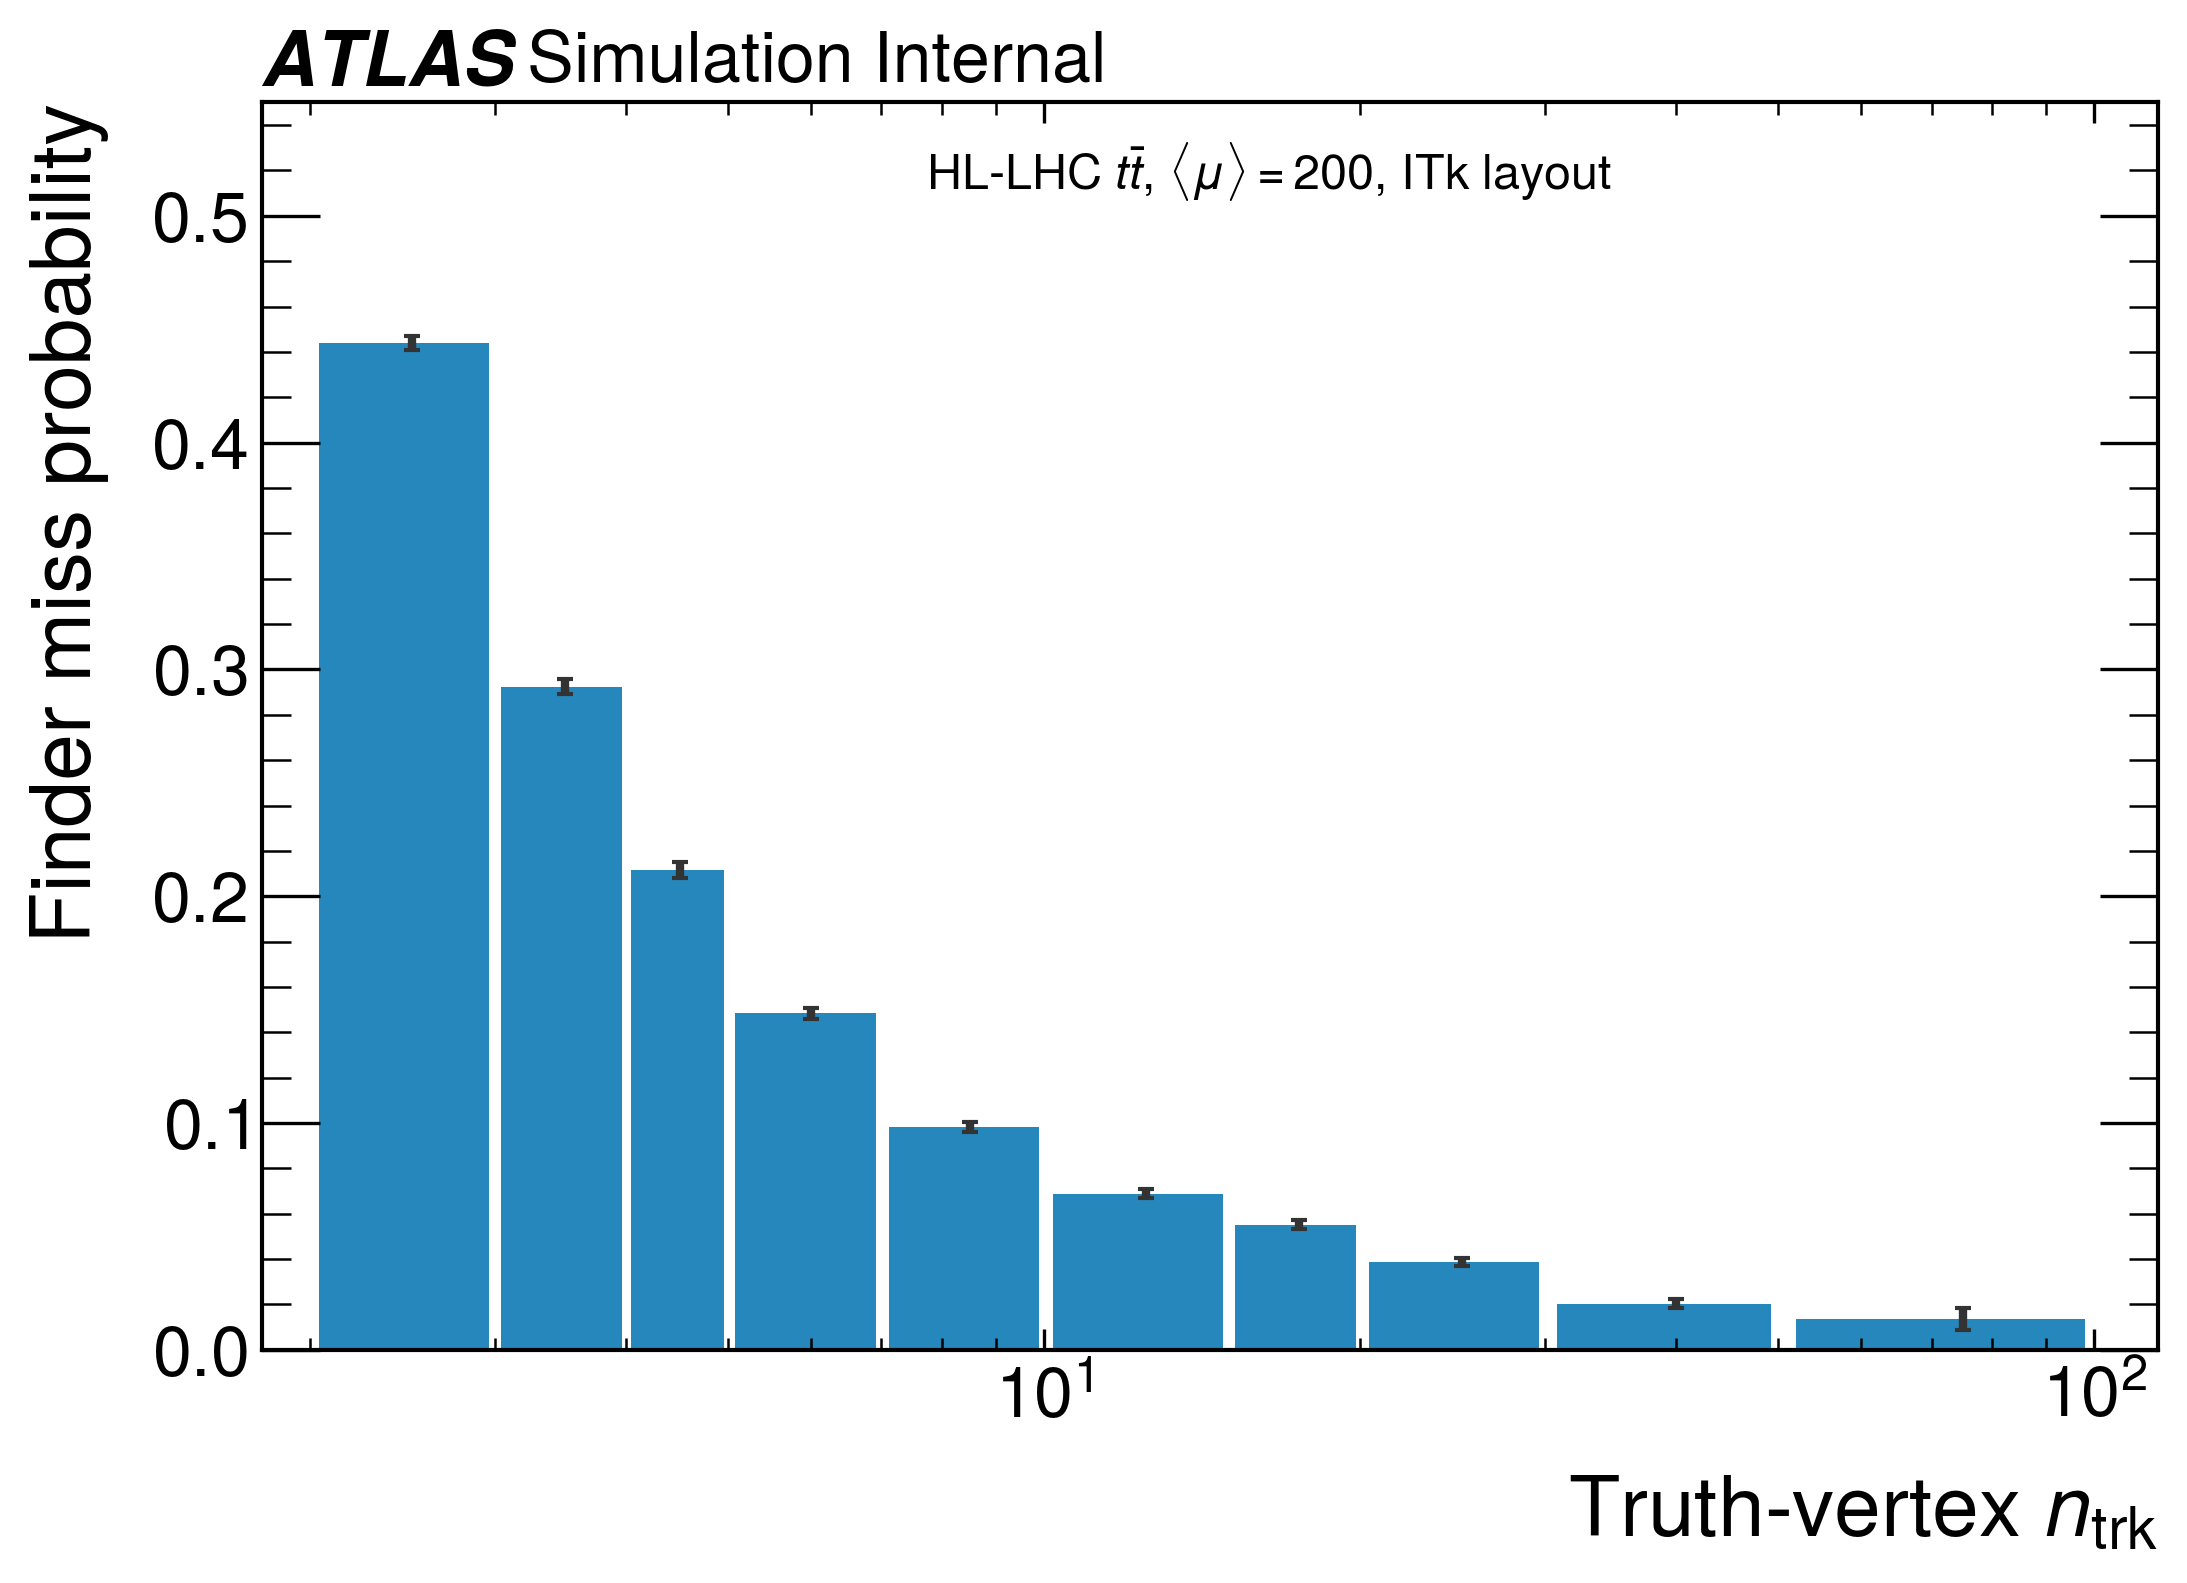
\includegraphics[width=0.6\linewidth, keepaspectratio]{images/pu200_miss_ntrk.png}\\[2pt]
    {\scriptsize\textcolor{black!55}{Probability that a truth vertex has no peak within 0.5~mm,
    vs its track multiplicity (PU200, v4b finder at the production operating point).}}
\end{frame}

\begin{frame}{HL-LHC Results}
    \begin{columns}
        \begin{column}{0.5\linewidth}
            \begin{figure}
                \centering
                \includegraphics[width=\linewidth]{images/resolution_plot_hl.png}
            \end{figure}
        \end{column}
        \begin{column}{0.5\linewidth}
            \begin{figure}
                \centering
                \includegraphics[width=\linewidth]{images/category_counts_hist_hl.png}
            \end{figure}
        \end{column}
    \end{columns}
\end{frame}

\begin{frame}{HL-LHC Results: Model Trained on Run 2 MC}
    \begin{columns}
        \begin{column}{0.5\linewidth}
            \begin{figure}
                \centering
                \includegraphics[width=\linewidth]{images/resolution_plot_hl_old_model.png}
            \end{figure}
        \end{column}
        \begin{column}{0.5\linewidth}
            \begin{figure}
                \centering
                \includegraphics[width=\linewidth]{images/category_counts_hist_hl_old_model.png}
            \end{figure}
        \end{column}
    \end{columns}
    \vspace{4pt}
    \centering
    \textit{Model trained on Run 2 MC performs pretty well too.}
\end{frame}

\begin{frame}{HL-LHC: What We've Done and What's Next}
    \begin{columns}[t]
        \begin{column}{0.48\linewidth}
            \textbf{What we've done:}
            \begin{enumerate}
                \setlength\itemsep{0.4em}
                \item Standard optimizations
                \item Warmup, learning rate decay
                \item Tried different model sizes
            \end{enumerate}
        \end{column}
        \begin{column}{0.52\linewidth}
            \textbf{Ideas to improve the model further:}
            \begin{itemize}
                \setlength\itemsep{0.4em}
                \item Increase UNet resolution
                \item Tweak model size
                \item Try different loss functions to focus on sidelobes in dense regions
                \item Improve peak finding algorithm
            \end{itemize}
        \end{column}
    \end{columns}
\end{frame}

\backupend

\end{document}
